%%%%%%%% ICML 2020 EXAMPLE LATEX SUBMISSION FILE %%%%%%%%%%%%%%%%%

\documentclass{article}

% Recommended, but optional, packages for figures and better typesetting:
\usepackage{amsmath,amsfonts,amssymb,amsthm}
\usepackage{microtype}
\usepackage{graphicx}
\usepackage{subfigure}
\usepackage{booktabs} % for professional tables
\usepackage{xr}
\usepackage{dsfont}
\usepackage{multirow}
\usepackage{multicol}
\usepackage{color, colortbl}
\usepackage{adjustbox}
\usepackage{xspace}
\usepackage{float}

\definecolor{Gray}{gray}{0.9}

\newcommand{\bs}{YOLO-joint}
\newcommand{\bbsshort}{YOLO-ft}
\newcommand{\bbs}{YOLO-ft-full}
\newcommand{\lstd}{LSTD(YOLO)}
\newcommand{\lstdfull}{LSTD(YOLO)-full}
\newcommand{\Ours}{Ours}
\newcommand{\weightmodule}{reweighting module }


% hyperref makes hyperlinks in the resulting PDF.
% If your build breaks (sometimes temporarily if a hyperlink spans a page)
% please comment out the following usepackage line and replace
% \usepackage{icml2020} with \usepackage[nohyperref]{icml2020} above.
\usepackage{hyperref}
% \hypersetup{colorlinks,allcolors=black}

% Attempt to make hyperref and algorithmic work together better:


\newcommand{\theHalgorithm}{\arabic{algorithm}}


\newcommand{\xin}[1]{\textcolor{red}{[Xin: #1]}}
\newcommand{\thomas}[1]{\textcolor{red}{[Thomas: #1]}}
\newcommand{\joey}[1]{\textcolor{blue}{[Joey: #1]}}
\newcommand{\fisher}[1]{\textcolor{blue}{[Fisher: #1]}}
\newcommand{\trevor}[1]{\textcolor{red}{[Trevor: #1]}}
\newcommand{\red}[1]{\textcolor{red}{#1}}

\newcommand{\model}{TFA\xspace}
\newcommand{\modelplural}{TFAs\xspace}
\renewcommand{\vec}[1]{\mathbf{#1}}
\newcommand\minisection[1]{\vspace{1mm}\noindent \textbf{#1}}
\newcommand{\rulesep}{\unskip\ \vrule\ }
\newcommand{\tablestyle}[2]{\setlength{\tabcolsep}{#1}\renewcommand{\arraystretch}{#2}\centering\footnotesize}

% \newcommand{\vec}[1]{\mathbf{#1}}


% Use the following line for the initial blind version submitted for review:
% \usepackage{icml2020}

% If accepted, instead use the following line for the camera-ready submission:
% \usepackage[accepted]{icml2020}

\usepackage[preprint]{icml2020}

% The \icmltitle you define below is probably too long as a header.
% Therefore, a short form for the running title is supplied here:
\icmltitlerunning{Frustratingly Simple Few-Shot Object Detection}

\begin{document}

\twocolumn[
\icmltitle{CS282 Machine Learning Report} % TD I edited out "approach to"

% It is OKAY to include author information, even for blind
% submissions: the style file will automatically remove it for you
% unless you've provided the [accepted] option to the icml2020
% package.

% List of affiliations: The first argument should be a (short)
% identifier you will use later to specify author affiliations
% Academic affiliations should list Department, University, City, Region, Country
% Industry affiliations should list Company, City, Region, Country

% You can specify symbols, otherwise they are numbered in order.
% Ideally, you should not use this facility. Affiliations will be numbered
% in order of appearance and this is the preferred way.
\icmlsetsymbol{equal}{*}

\begin{icmlauthorlist}
\icmlauthor{Junda Shen}{equal,to}
\icmlauthor{Zian He}{equal,to}
\end{icmlauthorlist}

\icmlaffiliation{to}{SIST, Shanghaitech University}

\icmlcorrespondingauthor{Junda Shen}{shenjd@shanghaitech.edu.cn}
\icmlcorrespondingauthor{Zian He}{heza@shanghaitech.edu.cn}
% \icmlcorrespondingauthor{Fisher Yu}{i@yf.io}

% You may provide any keywords that you
% find helpful for describing your paper; these are used to populate
% the "keywords" metadata in the PDF but will not be shown in the document
\icmlkeywords{Machine Learning, ICML}
\vskip 0.3in
]

% this must go after the closing bracket ] following \twocolumn[ ...

% This command actually creates the footnote in the first column
% listing the affiliations and the copyright notice.
% The command takes one argument, which is text to display at the start of the footnote.
% The \icmlEqualContribution command is standard text for equal contribution.
% Remove it (just {}) if you do not need this facility.

%\printAffiliationsAndNotice{}  % leave blank if no need to mention equal contribution
\begin{NoHyper}\printAffiliationsAndNotice{\icmlEqualContribution}\end{NoHyper}
%\printAffiliationsAndNotice{\icmlEqualContribution} % otherwise use the standard text.

\begin{abstract}
In this project, we try to conquer the few-shot object detection problem by fine-tuning the last layer of some existing convolutional object detectors, e.g. Faster-RCNN. The prior methods usually encounter high variance problems which made them unreliable. However, we used an elegant sampling method so that the results are stable and the overfitting problem is diminished. We evaluated our approach on COCO and LVIS datasets, which shows that our method outperforms prior methods by 2 ~ 15 percent. Since this method does not propose a new architecture, the code is based on and modified from the detectron2 package, you can find the original code at ~\url{https://github.com/facebookresearch/detectron2}.
\end{abstract}

\section{Introduction}
Nowadays, many tasks can be done by machine perception systems and learning from only a few samples has raised wide attention due to the scarcity of samples in some particular areas. Although some few-shot learning problems has almost been solved, it is still hard to achieve image detection with few training samples, the detection results are still unideal.

In the prior works, people have tried to achieve few-shot image detection by two approaches
\begin{enumerate}
    \item Meta-learning. This approach tries to transfer knowledge learnt from data-abundent classes to data-scarce novel classes so that the model could adapt to the new task more quickly. This method have been used in few-shot image classification for a while but it has not been proved effective in object detection task, which is much more challenging than image classification.
    \item Metric-learning. This approach tries to build some metrics for the learner so that it can estimate and check the similarities between images, e.g. cosine similarities. Based on the built metrics, the model can try to fit to the input and learn how to detect objects. However, this approach relis on the metric, which may be hard to find a better one.
\end{enumerate}

The object detection task is much harder than the image classification task, since it contains not only classification but also object localization. Researchers ~\cite{kang2019few,yan2019meta,wang2019meta} have attempted to achieve few-shot object detection task, where a few labeled data, far from abundent, is provided to the learner as novel training data. These methods achieved out-of-random performance but their methods are not stable, which means the reproduced results might be far from their reported results.

\begin{figure*}[ht]
    \centering
    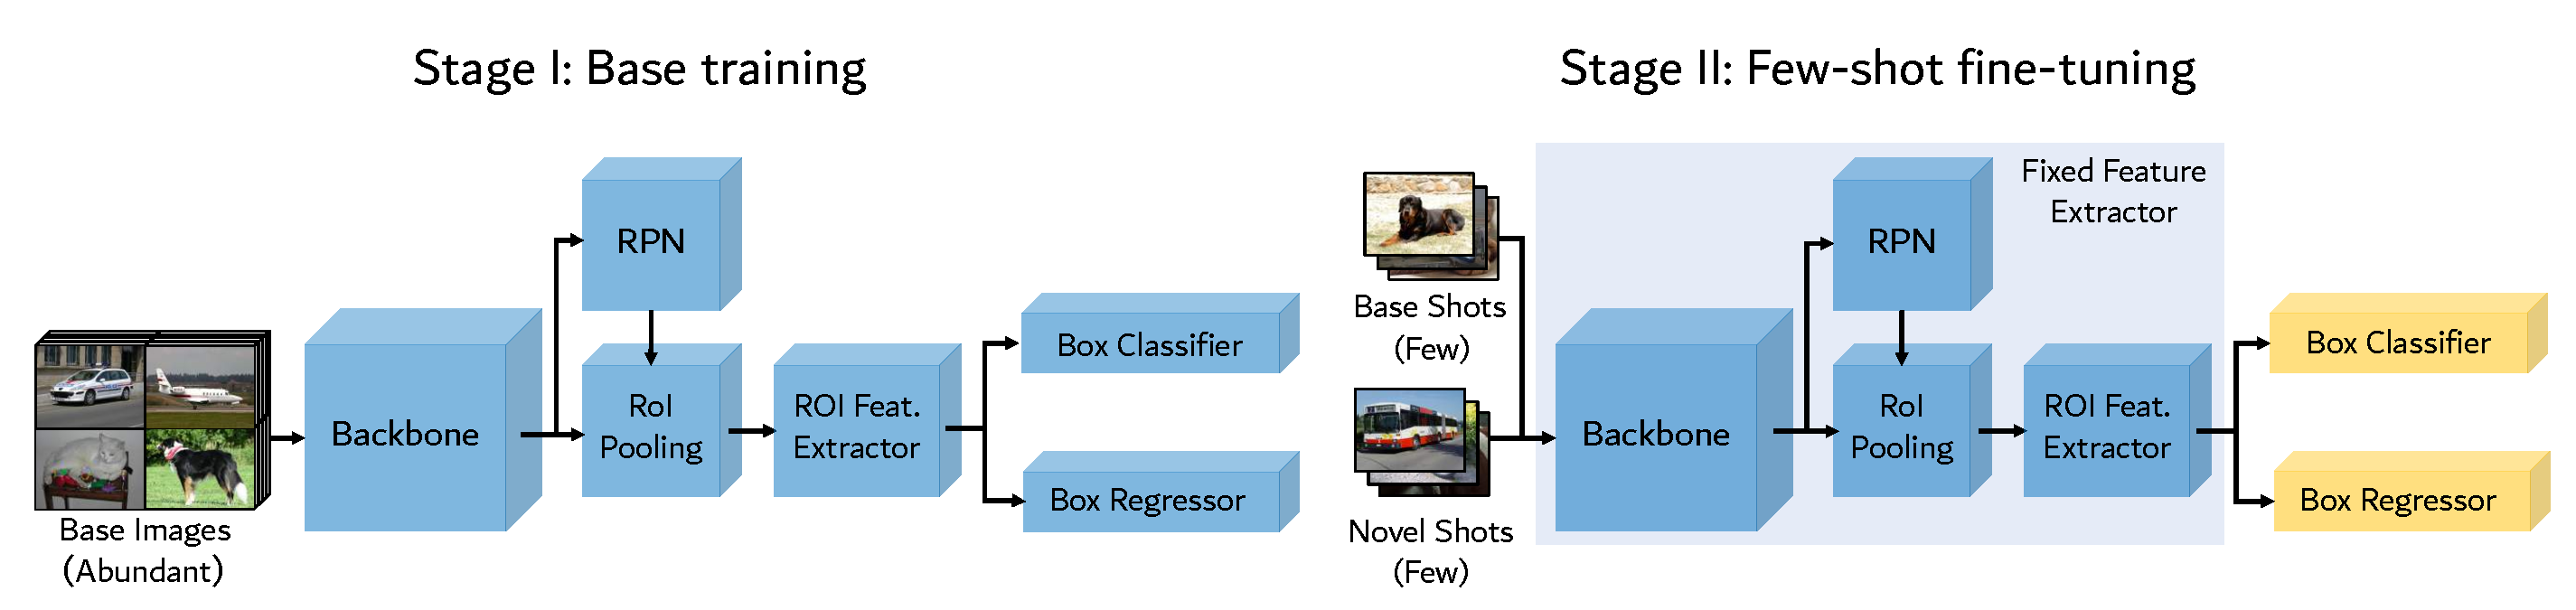
\includegraphics[width=\linewidth]{figs/TFA_fig1.pdf}
    \label{fig:tfa_arch}
    \vspace{-1cm}
    \caption{Illustration of our two-stage fine-tuning approach (\model). In the base training stage, the entire object detector, including both the feature extractor $\mathcal{F}$ and the box predictor, are jointly trained on the base classes. In the few-shot fine-tuning stage, the feature extractor components are fixed and only the box predictor is fine-tuned on a balanced subset consisting of both the base and novel classes.}
\end{figure*}

In this project, we try to improve the detection results by adopting fine-tuning based approaches. We focus on the schedule of the training procedure and use proper instance-level feature normalization in this project.

The training is composed of two stages, which is shown in Figure~\ref{fig:tfa_arch}. The first stage trains the whole network, e.g. Faster-RCNN, on data-abundent base classes. Then we only train the last layer of the network in the second stage, on a small balanced training set that is composed of both base and novel classes by properly sample data, parameters in other layers of the detector is kept intact during the second stage. We also use instance-level feature normalization in the second stage, which helps the model to diminish some parameter issues introduced by~\citet{gidaris2018dynamic,qi2018low,chen2019closer}.

In our evalution, we find that our method outperfroms all previous few-shot object detection methods, our method can gain 2 $\sim$ 15 percent more accuracy than prior methods, and it even doubled the accuracy in one-shot learning, which dictates the effiction of our method.

We fixed several issues in the existing training procedures
\begin{enumerate}
    \item We try to diminish overfitting by invoking multiple runs on different random samples so that the variance is lower and the results much are more stable.
    \item We try to keep the accuracy of our method consistent with the paper.
    \item We report not only the accuracy for novel classes, but also accuracy for base classes and the overall accuracy for all classes, so that one can see that the accuracy (referred to as the generalized few-shot learning setting in the few-shot classification literature~\cite{hariharan2017low,wang2019tafe}) for other classes are not largely affected.
\end{enumerate}

On the challenging LVIS dataset, our two-stage training scheme improves the average detection precision of rare classes
($<$10 images) by $\sim$4 points and common classes (10-100 images) by $\sim$2 points with negligible precision loss for the frequent classes ($>$100 images).

\section{Related Work}
Our work is related to the rich literature on few-shot image classification, which uses various 
meta-learning based or metric-learning based methods. We also draw connections between our work and the existing meta-learning based few-shot object detection methods. To the best of our knowledge, we are the first to conduct a systematic analysis of fine-tuning based approaches on few-shot object detection. 

\minisection{Meta-learning.} The goal of meta-learning is to acquire task-level meta knowledge that
can help the model quickly adapt to new tasks and environments with very few labeled examples.  Some~\cite{finn2017model,rusu2018meta,nichol2018reptile} learn to fine-tune and aim to obtain a good parameter initialization that can adapt to
new tasks with a few scholastic gradient updates. Another popular line of research on meta-learning is to use parameter generation during adaptation to novel tasks. \citet{gidaris2018dynamic} propose an attention-based weight generator to generate the classifier weights for the novel classes. \citet{wang2019tafe} construct task-aware feature embeddings by generating parameters for the feature layers. These approaches have only been used for few-shot image 
classification and not on more challenging tasks like object detection.

However, some~\cite{chen2019closer} 
raise concerns about the reliability of the results given 
that a consistent comparison of different approaches is missing. 
Some simple fine-tuning based approaches, which draw little attention in the
community, turn out to be more favorable than many prior works that use meta-learning
on few-shot image classification~\cite{chen2019closer,dhillon2019baseline}.
As for the emerging few-shot object detection task, there is neither consensus on the evaluation benchmarks nor a consistent comparison of different approaches due to the increased network complexity, obscure implementation details, and variances in evaluation protocols.

\minisection{Metric-learning.} Another line of work~\cite{koch2015siamese,snell2017prototypical,vinyals2016matching}
focuses on learning to compare or metric-learning. Intuitively, if the model can construct distance metrics to 
estimate the similarity between two input images, it may generalize to 
novel categories with few labeled instances. More recently, several~\cite{chen2019closer,gidaris2018dynamic,qi2018low} adopt a 
cosine similarity based classifier to reduce the intra-class variance on the few-shot classification task, which leads to favorable performance compared to many 
meta-learning based approaches. Our method also adopts a cosine
similarity classifier to classify the categories of the region proposals. However, we focus on the instance-level distance measurement rather than on the image level.

\minisection{Few-shot object detection.} There are several early attempts 
at few-shot object detection using meta-learning. ~\citet{kang2019few} and 
~\citet{yan2019meta} apply feature re-weighting schemes to a
single-stage object detector (YOLOv2) and a two-stage object detector
(Faster R-CNN), with the help of a meta learner that takes the support images (\textit{i.e.}, a small number of labeled images of the novel/base classes) 
as well as the bounding box annotations as inputs. ~\citet{wang2019meta} 
propose a weight prediction meta-model to predict parameters of
category-specific components from the few examples while learning the category-agnostic components from base class examples. 

In all these works, fine-tuning based approaches are considered as baselines
with worse performance than meta-learning based approaches. They consider
\emph{jointly fine-tuning}, where base classes and novel classes are trained together, and \emph{fine-tuning the entire model}, where the detector is first trained on the base classes only and then fine-tuned on a balanced set with both base and novel classes. In contrast, we find that fine-tuning only the last layer of the object detector on the balanced subset and keeping the rest of model fixed can substantially improve the
detection accuracy, outperforming all the prior meta-learning based
approaches. This indicates that feature representations
learned from the base classes might be able to transfer to the novel classes
and simple adjustments to the box predictor can provide 
strong performance gain~\cite{dhillon2019baseline}. 



\vspace{-0.3cm}
\section{Algorithms for Few-Shot Object Detection}

In this section, we first focus on the few-shot object detection setting. Then, we will show our two-stage fine-tuning approach in
Section~\ref{sec:tfa} and Section~\ref{sec:meta}.

\subsection{Task formalization}
There are two kinds of classes, one kind is base classes $C_b$ that have many instances and the other one is novel classes $C_n$ that have only $K$ (usually less than 10) instances per class.
For an object detection dataset $\mathcal{D}=\{(x, y), x\in\mathcal{X}, y\in\mathcal{Y}\}$ ($x$
is the input image, $y=\{(c_i, \vec{l}_i), i=1, ...,N\}$ denotes the categories $c \in C_b \cup C_n$
and bounding box coordinates $\vec{l}$ of the $N$ object instances in the image $x$). Now we will use the dataset $\mathcal{D}$ to learn categorie $c$ and the corresponding box corrdinates $l$ for each object and try to improve the detection accuracy.

\subsection{Two-stage fine-tuning approach}
\label{sec:tfa}
Our method (\model) including two stages, which is shown in Figure~\ref{fig:tfa_arch}. The base detection model is formed by Faster R-CNN~\cite{ren2015faster} and a two-stage object detector.

Since the features in the first few layers are class-agnostic, features learned from the base classes are likely to transfer to the novel classes with parameters fixed.

\minisection{Base model training.} In this stage, we train the network with large number of samples. The loss of the network consists of three parts,
\begin{equation}
    \mathcal{L} = \mathcal{L}_{\text{rpn}} + \mathcal{L}_{\text{cls}} + \mathcal{L}_{\text{loc}},
    \label{eq:loss}
\end{equation}
which are loss of the RPN network, cross-entropy loss for the box classifier and smoothed $L_1$ loss for the box regressor, respectively.

\minisection{Few-shot fine-tuning.} In this stage, we fine-tune the network based on rare samples. We keep the first few layers unchanged, assign random weights of the new class to the box predictior, and only fine-tune the last layer. We use the same loss function as the previous stage but decreases the learning rate by 20.

\begin{figure*}[ht]
    \centering
    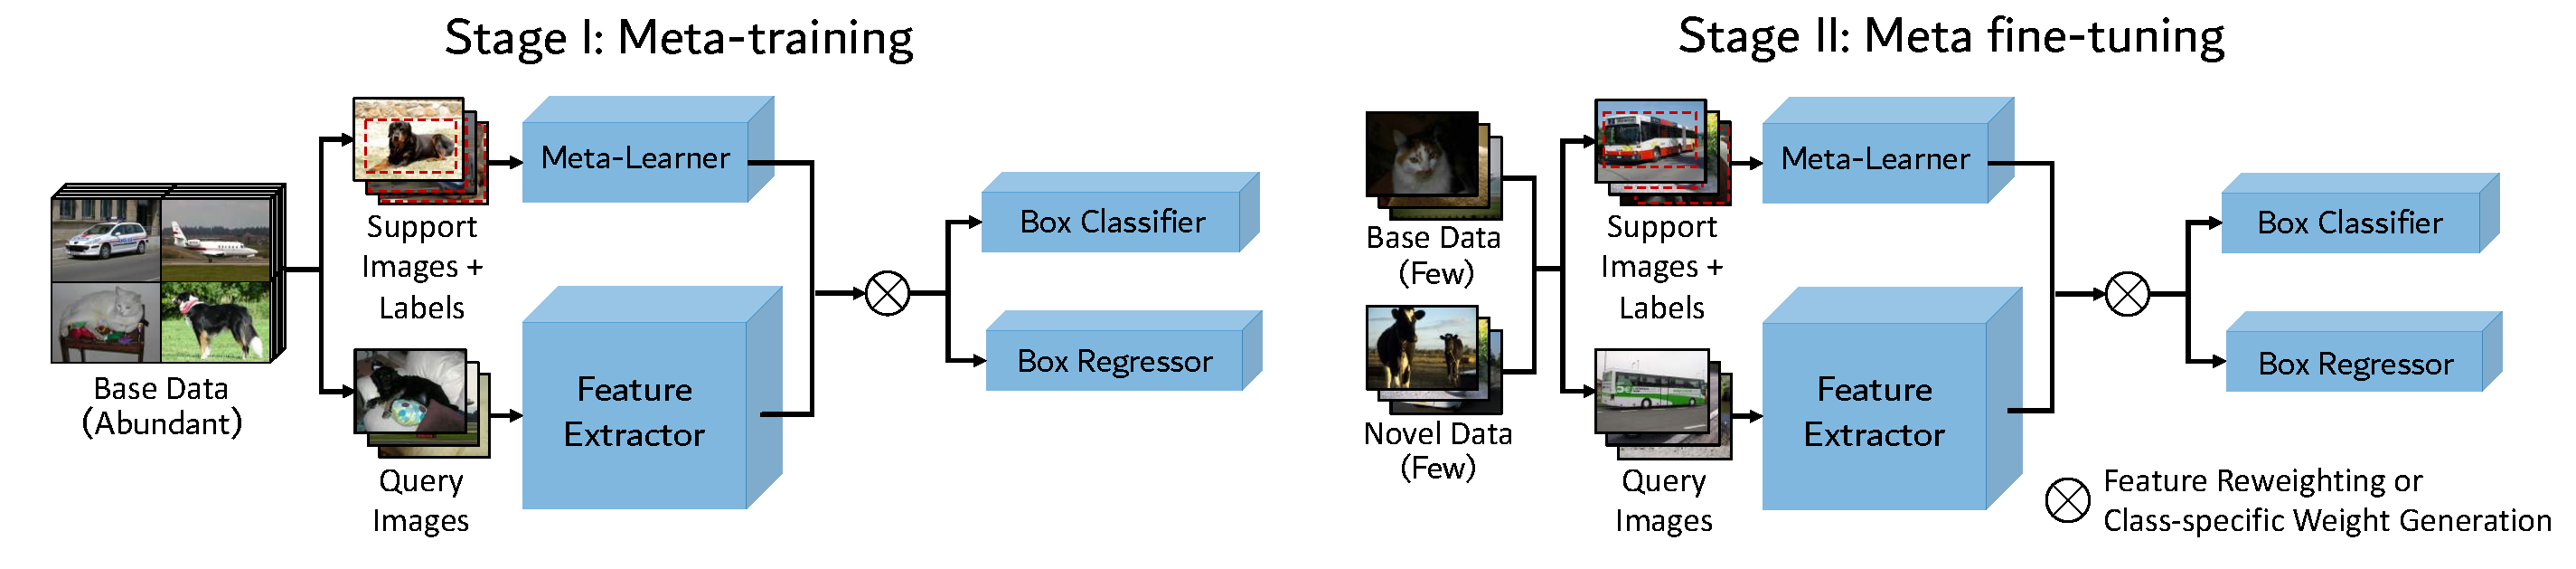
\includegraphics[width=\linewidth]{figs/TFA_fig2.pdf}
    \vspace{-8mm}
    \caption{Abstraction of the meta-learning based few-shot object detectors. A meta-learner is introduced to acquire task-level meta information and help the model generalize to novel classes through feature re-weighting (\textit{e.g.}, FSRW and Meta R-CNN) or weight generation (\textit{e.g.}, MetaDet). A two-stage training approach (meta-training and meta fine-tuning) with episodic learning is commonly adopted.}
    \label{fig:meta_arch}
\end{figure*}

\minisection{Cosine similarity for box classifier.} The design of the classifier is based on the cosine similarity function, inspired by ~\citet{gidaris2018dynamic,qi2018low,chen2019closer}.
The weight matrix of the box classifier is $W\in\mathbb{R}^{d\times c}$, where $w_c\in\mathbb{R}^d$ is the per-class weight vector. The output of $\mathcal{C}$ is scaled similarity scores $S$
\begin{equation}
    s_{i,j} = \frac{\alpha \mathcal{F}(x)_i^\top w_j}{\|\mathcal{F}(x)_i\| \|w_j\|},
    \label{eq:classifier} 
\end{equation}
where $s_{i,j}$ is the similarity calculated between the $i$-th proposed object and the weight vector of class $j$. $\alpha$ is a scaling factor. We use a fixed $\alpha$ of 20 and use instance-level feature normalization in our experiments to help diminish the variance.

\subsection{Compared Meta-learning with Fine-tuning}
\label{sec:meta}
Both the meta-learning method and our method are composed of two stages. However, since our fine-tuning method only fine-tunes the last layer of the network, our method is much more memory efficient than the meta-learning method.

\section{Experiments}

We evaluate our method on two datasets
\begin{enumerate}
	\item COCO
	\item LVIS
\end{enumerate}
We then provide some quantitative results and visualization results in this section.

\minisection{Implementation details.}
We select Faster R-CNN~\cite{ren2015faster} as our base detector and use Resnet-101~\cite{he2016deep} with a Feature Pyramid Network~\cite{lin2016feature} as the backbone of our method.
All models are trained using SGD with a mini-batch size of 16, momentum of 0.9, and weight decay of 0.0001. A learning rate of 0.02 is used during base training and 0.001 during few-shot fine-tuning. 
For hyperparameters related to the model architecture, we use the default parameters provided by Detectron2.

\subsection{Existing few-shot object detection benchmark}
\label{sec:exist_benchmark}
% We first evaluate our approach on two existing few-shot object detection benchmarks, PASCAL VOC \cite{pascal-voc-2007, pascal-voc-2012} and COCO \cite{Lin2014MicrosoftCC}.
% We use the same evaluation protocol as previous works \cite{kang2019few, yan2019meta, wang2019meta}, which we will describe next.
\minisection{Existing benchmarks.} 
Following the previous work~\cite{kang2019few,yan2019meta,wang2019meta}, we 
first evaluate our approach on COCO, using the same data splits and training examples provided by ~\citet{kang2019few}.
% \footnote{code and data at \url{https://github.com/bingykang/Fewshot_Detection}}. 
For COCO, the 60 categoriesare used as base classes while the remaining 20 classes are used as novel classes with $K=10, 30$.  For evaluation metrics, the COCO-style AP of the novel classes is used on COCO. 
% On PASCAL VOC, we use the train/val sets in VOC 2007 and 2012 for training and the VOC 2007 test set for evaluation.
% To construct the few-shot setting, we randomly split the 20 object categories into 15 as the base categories and the remaining 5 as the novel categories, and we evaluate on three different random splits.
% On COCO, we use 5k images from the validation set for evaluation and the remaining images from the train/val sets for training.
% From the 80 object categories, we set the same 20 categories as in PASCAL VOC as the novel categories and the remaining 60 as the base categories.
% On PASCAL VOC, we set the number of shots, $K$, to 1, 2, 3, 5, and 10.
% On COCO, $K$ is set to 10 and 30.  

\minisection{Baselines.} We compare our approach with the meta-learning approaches \texttt{FSRW}, \texttt{Meta-RCNN} and \texttt{MetaDet} together with the fine-tuning
based approaches:  \emph{jointly training}, denoted by \texttt{FRCN/YOLO+joint}, where the base and novel class examples are jointly trained in one stage,  and \emph{fine-tuning the entire model}, denoted by \texttt{FRCN/YOLO+ft-full}, where both the feature extractor $\mathcal{F}$ and the box predictor ($\mathcal{C}$ and $\mathcal{R}$) are jointly fine-tuned until convergence in the second fine-tuning stage. \texttt{FRCN} is Faster R-CNN for short. Fine-tuning with less iterations, denoted by \texttt{FRCN/YOLO+ft}, are reported in ~\citet{kang2019few} and ~\citet{yan2019meta}.

% We compare our approach to several baseline methods.
% % \textit{FRCN+joint} jointly trains the object detector on data from both the base categories and the novel categories.
% \textit{FRCN+ft} also uses a two-stage training scheme, but fine-tunes the entire model instead of just the predictor.
% We train this baseline with the same number of iterations as our method.
% We also compare our approach to previous meta-learning based methods, FSRW~\cite{kang2019few}, MetaDet~\cite{wang2019meta}, and Meta R-CNN~\cite{yan2019meta}.


% The main evaluation results on PASCAL VOC are shown in Table~\ref{tab:main_voc}.
% Our approach consistently outperforms previous methods by a large margin across all three splits and across all shots.
% The improvements are greatest when the number of shots are low.
% On 1 shot, our approach sometimes even doubles the mAP50 of previous methods.
% % In contrast, the performance of \textit{FRCN+joint} is significantly worse.
% % This shows the important of using a two-stage training scheme, or else the training data will be dominated by the base categories and the detector will not learn anything about the novel categories.
% In constrast, the performance of \textit{FRCN+ft} is much worse, which shows the importance of separating the learning of the predictor and the feature extractor.

\begin{table}[ht]
    \centering
    \footnotesize
    % \vspace{-5mm}
\caption{{Few-shot detection performance for the novel categories on the COCO dataset.} Our approach consistently outperforms baseline methods across all shots and metrics.\vspace{2mm}}
    \adjustbox{width=\linewidth}{
    \begin{tabular}{l|cc|cc}
    \toprule
    \multirow{2}{*}{Model} %&\multirow{2}{*}{Backbone}
    &\multicolumn{2}{c|}{novel AP} & \multicolumn{2}{c}{novel AP75}\\
    & 10 & 30 & 10 & 30 \\ \midrule
    FSRW\small{~\cite{kang2019few}}  & 5.6 & 9.1 & 4.6 & 7.6 \\ 
    MetaDet\small{~\cite{wang2019meta}} & 7.1 & 11.3 & 6.1 & 8.1 \\
    FRCN+ft+full\small{~\cite{yan2019meta}} &  6.5 & 11.1 & 5.9 & 10.3\\
    Meta R-CNN\small{~\cite{yan2019meta}}  & 8.7 & 12.4 & 6.6 & 10.8\\ % \midrule
    FRCN+ft-full (Our Impl.)  & 9.2 & 12.5  & 9.2 & 12.0  \\ 	
    \rowcolor{Gray} \model w/ fc (Ours)  & \textbf{10.0} & 13.4  & 9.2 & 13.2 \\
    \rowcolor{Gray} \model w/ cos (Ours) & \textbf{10.0} & \textbf{13.7}  & \textbf{9.3} & \textbf{13.4}\\
    \bottomrule
    \end{tabular}}
\label{tab:main_coco}
% \vspace{-5mm}
\end{table}

\minisection{Results on COCO.} Similarly, we report the average AP and AP75 of the 20 novel classes on COCO in Table~\ref{tab:main_coco}. AP75 means matching threshold is 0.75, a more strict metric than AP50. Again, we consistently outperform previous methods across all shots on both novel AP and
novel AP75. We achieve around 1 point improvement in AP over the best performing baseline and around 2.5 points improvement in AP75.

\begin{table*}[t]
	\centering
	\footnotesize
	\setlength{\tabcolsep}{0.4em}
	\caption{Generalized object detection benchmarks on LVIS. We compare our approach to the baselines provided in LVIS~\cite{gupta2019lvis}. Our approach outperforms the corresponding baseline across all metrics, backbones, and sampling schemes. \vspace{1mm}}
	\adjustbox{width=.8\linewidth}{
		\begin{tabular}{c|c|c|ccc|ccc|ccc}
			\toprule
			Method & Backbone  & Repeated sampling & AP & AP50 & AP75 & APs & APm & APl & APr & APc & APf \\\midrule
			Joint training~\cite{gupta2019lvis}  & \multirow{3}{*}{FRCN w/ R-50} && 19.8 & 33.6 & 20.4 & 17.1 & 25.9 & 33.2 & 2.1 & 18.5 & \textbf{28.5}  \\
			\model w/ fc (Ours) &  &  & 22.6 & 37.5 & 22.6 & 17.5 & 27.2 & 36.3 & 14.2 & 21.0 & 26.8 \\
			\model w/ cos (Ours) &  &  & \cellcolor{Gray} 22.9 & \cellcolor{Gray} 37.5 & \cellcolor{Gray} 23.6 & \cellcolor{Gray} 19.0 & \cellcolor{Gray} 27.5 & \cellcolor{Gray} 37.0 & \cellcolor{Gray} 15.5 & \cellcolor{Gray} 20.8 & \cellcolor{Gray} 27.9 \\ \midrule
			Joint training~\cite{gupta2019lvis}  & \multirow{3}{*}{FRCN w/ R-50}  &\multirow{3}{*}{\checkmark} & 23.1 & 38.4 & 24.3 & 18.1 & 28.3 & 36.0 & 13.0 & 22.0 & 28.4 \\ 
			\model w/ fc (Ours) &  & & 24.0 & 40.0 & 26.0 & 19.3 & 28.9 & 36.5 & 15.0 & 24.1 & 28.1 \\
			\model w/ cos (Ours) & &&\cellcolor{Gray} \textbf{24.5} & \cellcolor{Gray}\textbf{40.2} & \cellcolor{Gray}\textbf{26.4} & \cellcolor{Gray}\textbf{20.1} & \cellcolor{Gray}\textbf{29.5} & \cellcolor{Gray}\textbf{38.5} &\cellcolor{Gray}\textbf{17.1} & \cellcolor{Gray}\textbf{24.5} & \cellcolor{Gray}27.8 \\ \midrule\midrule
			Joint training~\cite{gupta2019lvis}  & \multirow{3}{*}{FRCN w/ R-101} & & 21.9 & 35.8 & 23.0 & 18.8 & 28.0 & 36.2 & 3.0 & 20.8 & \textbf{30.8}  \\
			\model w/ fc (Ours) &  & & 24.0 & 39.2 & 25.1 & 19.2 & 29.8 & 38.8 & 15.8 & 22.7 & 29.1  \\
			\model w/ cos (Ours) &  & & \cellcolor{Gray} 24.5 & \cellcolor{Gray} 39.6 & \cellcolor{Gray} 26.0 & \cellcolor{Gray} 20.3 & \cellcolor{Gray} 30.6 & \cellcolor{Gray} 39.8 & \cellcolor{Gray} \textbf{18.3} & \cellcolor{Gray} 21.5 & \cellcolor{Gray} 30.1
  \\\midrule
			Joint training~\cite{gupta2019lvis} & \multirow{3}{*}{FRCN w/ R-101}  & \multirow{3}{*}{\checkmark} & 24.7 & 40.5 & 26.0 & 19.0 & 30.3 & 38.0 & 13.4 & 24.0 & 30.1 \\ 
			\model w/ fc (Ours) &  & & 25.6 & \textbf{41.8} & 26.8 & 20.0 & 31.0 & 39.3 & 15.7 & 26.1 & 28.3 \\
			\model w/ cos (Ours) & & & \cellcolor{Gray} \textbf{26.5} & \cellcolor{Gray}\textbf{41.9} & \cellcolor{Gray}\textbf{27.6} & \cellcolor{Gray}\textbf{20.1} & \cellcolor{Gray}\textbf{32.2} & \cellcolor{Gray}\textbf{40.0} & \cellcolor{Gray}17.2 & \cellcolor{Gray}\textbf{26.3} & \cellcolor{Gray}29.8 \\ 
			\bottomrule
	\end{tabular}}
	\label{tab:lvis_bench}
\end{table*}


% \begin{table*}[!h]
% \centering
% \footnotesize
% \setlength{\tabcolsep}{0.4em}
% \caption{Generalized object detection benchmarks on Pascal VOC. For each metric, we report the average and 95\% confidence interval computed over 30 random samples. \vspace{1mm}}
% \adjustbox{width=.9\linewidth}{
% \begin{tabular}{c|c|c|ccc|ccc|ccc}
% \toprule
% \multirow{2}{*}{Split} & \multirow{2}{*}{\# shots} &\multirow{2}{*}{Method} &  \multicolumn{3}{c|}{Overall}  &\multicolumn{3}{c|}{Base class} & \multicolumn{3}{c}{Novel class} \\ \cmidrule{4-12}
% & & & AP & AP50 & AP75 & bAP & bAP50 & bAP75 & nAP & nAP50 & nAP75 \\ \midrule
% \multirow{12}{*}{Split 1} & \multirow{2}{*}{1} & \model w/ fc & 39.6$\pm$0.5 & 63.5$\pm$0.7 & 43.2$\pm$0.7 & 48.7$\pm$0.7 & 77.1$\pm$0.7 & 53.7$\pm$1.0 & 12.2$\pm$1.6 & 22.9$\pm$2.5 & 11.6$\pm$1.9 \\
%     & &\cellcolor{Gray} \model w/ cos & \cellcolor{Gray}40.6$\pm$0.5 & \cellcolor{Gray}64.5$\pm$0.6 & \cellcolor{Gray}44.7$\pm$0.6 & \cellcolor{Gray}49.4$\pm$0.4 & \cellcolor{Gray}77.6$\pm$0.2 & \cellcolor{Gray}54.8$\pm$0.5 & \cellcolor{Gray}14.2$\pm$1.4 &\cellcolor{Gray} 25.3$\pm$2.2 & \cellcolor{Gray}14.2$\pm$1.8 \\ \cmidrule{2-12}
%     & \multirow{2}{*}{2} & \model w/ fc & 40.5$\pm$0.5 & 65.5$\pm$0.7 & 43.8$\pm$0.7 & 47.8$\pm$0.7 & 75.8$\pm$0.7 & 52.2$\pm$1.0 & 18.9$\pm$1.5 & 34.5$\pm$2.4 & 18.4$\pm$1.9  \\
%     & &\cellcolor{Gray} \model w/ cos & \cellcolor{Gray}42.6$\pm$0.3 & \cellcolor{Gray} 67.1$\pm$0.4 & \cellcolor{Gray}47.0$\pm$0.4 &\cellcolor{Gray} 49.6$\pm$0.3 & \cellcolor{Gray}77.3$\pm$0.2 & \cellcolor{Gray}55.0$\pm$0.4 & \cellcolor{Gray}21.7$\pm$1.0 & \cellcolor{Gray}36.4$\pm$1.6 & \cellcolor{Gray}22.8$\pm$1.3  \\ \cmidrule{2-12}
%     & \multirow{2}{*}{3} & \model w/ fc & 41.8$\pm$0.9 & 67.1$\pm$0.9 & 45.4$\pm$1.2 & 48.2$\pm$0.9 & 76.0$\pm$0.9 & 53.1$\pm$1.2 & 22.6$\pm$1.2 & 40.4$\pm$1.7 & 22.4$\pm$1.7  \\
%     & & \cellcolor{Gray}\model w/ cos &\cellcolor{Gray} 43.7$\pm$0.3 &\cellcolor{Gray} 68.5$\pm$0.4 & \cellcolor{Gray}48.3$\pm$0.4 & \cellcolor{Gray}49.8$\pm$0.3 & \cellcolor{Gray}77.3$\pm$0.2 & \cellcolor{Gray}55.4$\pm$0.4 & \cellcolor{Gray}25.4$\pm$0.9 & \cellcolor{Gray}42.1$\pm$1.5 & \cellcolor{Gray}27.0$\pm$1.2  \\ \cmidrule{2-12}
%     & \multirow{2}{*}{5} & \model w/ fc & 41.9$\pm$0.6 & 68.0$\pm$0.7 & 45.0$\pm$0.8 & 47.2$\pm$0.6 & 75.1$\pm$0.6 & 51.5$\pm$0.8 & 25.9$\pm$1.0 & 46.7$\pm$1.4 & 25.3$\pm$1.2  \\
%     & &\cellcolor{Gray} \model w/ cos &\cellcolor{Gray} 44.8$\pm$0.3 & \cellcolor{Gray}70.1$\pm$0.4 &\cellcolor{Gray} 49.4$\pm$0.4 &\cellcolor{Gray} 50.1$\pm$0.2 &\cellcolor{Gray} 77.4$\pm$0.3 &\cellcolor{Gray} 55.6$\pm$0.3 &\cellcolor{Gray} 28.9$\pm$0.8 & \cellcolor{Gray}47.9$\pm$1.2 & \cellcolor{Gray}30.6$\pm$1.0  \\ \cmidrule{2-12}
%     & \multirow{2}{*}{10} & \model w/ fc & 42.8$\pm$0.3 & 69.5$\pm$0.4 & 46.0$\pm$0.4 & 47.3$\pm$0.3 & 75.4$\pm$0.3 & 51.6$\pm$0.4 & 29.3$\pm$0.7 & 52.0$\pm$1.1 & 29.0$\pm$0.9  \\
%     & &\cellcolor{Gray} \model w/ cos & \cellcolor{Gray}45.8$\pm$0.2 & \cellcolor{Gray}71.3$\pm$0.3 & \cellcolor{Gray}50.4$\pm$0.3 &\cellcolor{Gray} 50.4$\pm$0.2 & \cellcolor{Gray}77.5$\pm$0.2 &\cellcolor{Gray} 55.9$\pm$0.3 & \cellcolor{Gray}32.0$\pm$0.6 & \cellcolor{Gray}52.8$\pm$1.0 & \cellcolor{Gray}33.7$\pm$0.7  \\ \midrule
% \multirow{12}{*}{Split 2} & \multirow{2}{*}{1} & \model w/ fc & 36.2$\pm$0.8 & 59.6$\pm$0.9 & 38.7$\pm$1.0 & 45.6$\pm$0.9 & 73.8$\pm$0.9 & 49.4$\pm$1.2 & 8.1$\pm$1.2 & 16.9$\pm$2.3 & 6.6$\pm$1.1  \\
%     & &\cellcolor{Gray} \model w/ cos & \cellcolor{Gray}36.7$\pm$0.6 &\cellcolor{Gray} 59.9$\pm$0.8 &\cellcolor{Gray} 39.3$\pm$0.8 &\cellcolor{Gray} 45.9$\pm$0.7 & \cellcolor{Gray}73.8$\pm$0.8 &\cellcolor{Gray} 49.8$\pm$1.1 & \cellcolor{Gray}9.0$\pm$1.2 & \cellcolor{Gray}18.3$\pm$2.4 &\cellcolor{Gray} 7.8$\pm$1.2 \\ \cmidrule{2-12}
%     & \multirow{2}{*}{2} & \model w/ fc & 38.5$\pm$0.5 & 62.8$\pm$0.6 & 41.2$\pm$0.6 & 46.9$\pm$0.5 & 74.9$\pm$0.5 & 51.2$\pm$0.7 & 13.1$\pm$1.0 & 26.4$\pm$1.9 & 11.3$\pm$1.1  \\
%     & & \cellcolor{Gray}\model w/ cos & \cellcolor{Gray}39.0$\pm$0.4 & \cellcolor{Gray}63.0$\pm$0.5 & \cellcolor{Gray}42.1$\pm$0.6 & \cellcolor{Gray}47.3$\pm$0.4 & \cellcolor{Gray}74.9$\pm$0.4 &\cellcolor{Gray} 51.9$\pm$0.7 &\cellcolor{Gray} 14.1$\pm$0.9 &\cellcolor{Gray} 27.5$\pm$1.6 &\cellcolor{Gray} 12.7$\pm$1.0  \\ \cmidrule{2-12}
%     & \multirow{2}{*}{3} & \model w/ fc & 39.4$\pm$0.4 & 64.2$\pm$0.5 & 42.0$\pm$0.5 & 47.5$\pm$0.4 & 75.4$\pm$0.5 & 51.7$\pm$0.6 & 15.2$\pm$0.8 & 30.5$\pm$1.5 & 13.1$\pm$0.8  \\
%     & & \cellcolor{Gray}\model w/ cos & \cellcolor{Gray}40.1$\pm$0.3 &\cellcolor{Gray} 64.5$\pm$0.5 &\cellcolor{Gray} 43.3$\pm$0.4 &\cellcolor{Gray} 48.1$\pm$0.3 & \cellcolor{Gray}75.6$\pm$0.4 & \cellcolor{Gray}52.9$\pm$0.5 & \cellcolor{Gray}16.0$\pm$0.8 & \cellcolor{Gray}30.9$\pm$1.6 & \cellcolor{Gray}14.4$\pm$0.9  \\ \cmidrule{2-12}
%     & \multirow{2}{*}{5} & \model w/ fc & 40.0$\pm$0.4 & 65.1$\pm$0.5 & 42.6$\pm$0.5 & 47.5$\pm$0.4 & 75.3$\pm$0.5 & 51.6$\pm$0.5 & 17.5$\pm$0.7 & 34.6$\pm$1.1 & 15.5$\pm$0.9  \\
%     & & \cellcolor{Gray}\model w/ cos & \cellcolor{Gray}40.9$\pm$0.4 & \cellcolor{Gray}65.7$\pm$0.5 & \cellcolor{Gray}44.1$\pm$0.5 & \cellcolor{Gray}48.6$\pm$0.4 &\cellcolor{Gray} 76.2$\pm$0.4 & \cellcolor{Gray}53.3$\pm$0.5 & \cellcolor{Gray}17.8$\pm$0.8 &\cellcolor{Gray} 34.1$\pm$1.4 & \cellcolor{Gray}16.2$\pm$1.0  \\ \cmidrule{2-12}
%     & \multirow{2}{*}{10} & \model w/ fc & 41.3$\pm$0.2 & 67.0$\pm$0.3 & 44.0$\pm$0.3 & 48.3$\pm$0.2 & 76.1$\pm$0.3 & 52.7$\pm$0.4 & 20.2$\pm$0.5 & 39.7$\pm$0.9 & 18.0$\pm$0.7  \\
%     & & \cellcolor{Gray}\model w/ cos & \cellcolor{Gray}42.3$\pm$0.3 &\cellcolor{Gray} 67.6$\pm$0.4 &\cellcolor{Gray} 45.7$\pm$0.3 &\cellcolor{Gray} 49.4$\pm$0.2 & \cellcolor{Gray}76.9$\pm$0.3 & \cellcolor{Gray}54.5$\pm$0.3 &\cellcolor{Gray} 20.8$\pm$0.6 &\cellcolor{Gray} 39.5$\pm$1.1 & \cellcolor{Gray}19.2$\pm$0.6  \\ \midrule
% \multirow{12}{*}{Split 3} & \multirow{2}{*}{1} & \model w/ fc & 39.0$\pm$0.6 & 62.3$\pm$0.7 & 42.1$\pm$0.8 & 49.5$\pm$0.8 & 77.8$\pm$0.8 & 54.0$\pm$1.0 & 7.8$\pm$1.1 & 15.7$\pm$2.1 & 6.5$\pm$1.0 \\
%     & & \cellcolor{Gray}\model w/ cos & \cellcolor{Gray}40.1$\pm$0.3 &\cellcolor{Gray} 63.5$\pm$0.6 &\cellcolor{Gray} 43.6$\pm$0.5 &\cellcolor{Gray} 50.2$\pm$0.4 & \cellcolor{Gray}78.7$\pm$0.2 & \cellcolor{Gray}55.1$\pm$0.5 & \cellcolor{Gray}9.6$\pm$1.1 & \cellcolor{Gray}17.9$\pm$2.0 &\cellcolor{Gray} 9.1$\pm$1.2  \\ \cmidrule{2-12}
%     & \multirow{2}{*}{2} & \model w/ fc & 41.1$\pm$0.6 & 65.1$\pm$0.7 & 44.3$\pm$0.7 & 50.1$\pm$0.7 & 77.7$\pm$0.7 & 54.8$\pm$0.9 & 14.2$\pm$1.2 & 27.2$\pm$2.0 & 12.6$\pm$1.3  \\
%     & & \cellcolor{Gray}\model w/ cos & \cellcolor{Gray}41.8$\pm$0.4 &\cellcolor{Gray} 65.6$\pm$0.6 &\cellcolor{Gray} 45.3$\pm$0.4 & \cellcolor{Gray}50.7$\pm$0.3 & \cellcolor{Gray}78.4$\pm$0.2 & \cellcolor{Gray}55.6$\pm$0.4 & \cellcolor{Gray}15.1$\pm$1.3 &\cellcolor{Gray} 27.2$\pm$2.1 & \cellcolor{Gray}14.4$\pm$1.5  \\ \cmidrule{2-12}
%     & \multirow{2}{*}{3} & \model w/ fc & 40.4$\pm$0.5 & 65.4$\pm$0.7 & 43.1$\pm$0.7 & 47.8$\pm$0.5 & 75.6$\pm$0.5 & 52.1$\pm$0.7 & 18.1$\pm$1.0 & 34.7$\pm$1.6 & 16.2$\pm$1.3  \\
%     & &\cellcolor{Gray} \model w/ cos &\cellcolor{Gray} 43.1$\pm$0.4 & \cellcolor{Gray}67.5$\pm$0.5 & \cellcolor{Gray}46.7$\pm$0.5 & \cellcolor{Gray}51.1$\pm$0.3 &\cellcolor{Gray} 78.6$\pm$0.2 &\cellcolor{Gray} 56.3$\pm$0.4 & \cellcolor{Gray}18.9$\pm$1.1 &\cellcolor{Gray} 34.3$\pm$1.7 &\cellcolor{Gray} 18.1$\pm$1.4  \\ \cmidrule{2-12}
%     & \multirow{2}{*}{5} & \model w/ fc & 41.3$\pm$0.5 & 67.1$\pm$0.6 & 44.0$\pm$0.6 & 48.0$\pm$0.5 & 75.8$\pm$0.5 & 52.2$\pm$0.6 & 21.4$\pm$0.9 & 40.8$\pm$1.3 & 19.4$\pm$1.0  \\
%     & & \cellcolor{Gray}\model w/ cos & \cellcolor{Gray}44.1$\pm$0.3 &\cellcolor{Gray} 69.1$\pm$0.4 & \cellcolor{Gray}47.8$\pm$0.4 & \cellcolor{Gray}51.3$\pm$0.2 & \cellcolor{Gray}78.5$\pm$0.3 & \cellcolor{Gray}56.4$\pm$0.3 & \cellcolor{Gray}22.8$\pm$0.9 & \cellcolor{Gray}40.8$\pm$1.4 & \cellcolor{Gray}22.1$\pm$1.1  \\ \cmidrule{2-12}
%     & \multirow{2}{*}{10} & \model w/ fc & 42.2$\pm$0.4 & 68.3$\pm$0.5 & 44.9$\pm$0.6 & 48.5$\pm$0.4 & 76.2$\pm$0.4 & 52.9$\pm$0.5 & 23.3$\pm$0.8 & 44.6$\pm$1.1 & 21.0$\pm$1.2  \\
%     & & \cellcolor{Gray}\model w/ cos & \cellcolor{Gray}45.0$\pm$0.3 & \cellcolor{Gray}70.3$\pm$0.4 &\cellcolor{Gray} 48.9$\pm$0.4 &\cellcolor{Gray} 51.6$\pm$0.2 &\cellcolor{Gray} 78.6$\pm$0.2 &\cellcolor{Gray} 57.0$\pm$0.3 & \cellcolor{Gray}25.4$\pm$0.7 & \cellcolor{Gray}45.6$\pm$1.1 & \cellcolor{Gray}24.7$\pm$1.1  \\
% \bottomrule
% \end{tabular}}
% \label{tab:voc_bench}
% \end{table*}



\subsection{Generalized few-shot object detection benchmark}
\label{sec:revised_bench}
% We now evaluate our approach on our new benchmarks for generalized few-shot object detection on three datasets: PASCAL VOC, COCO, and LVIS ~\cite{gupta2019lvis}.
% We first discuss the revisions we make to the existing benchmarks and then present our results.
\minisection{Revised evaluation protocols.}
% \xin{say something like we find the issues with the existing metrics; (1) generalized setting. The previous benchmark evaluates the novel and base classes, which can not effectively evaluate the performance drop in base classes and the overall performance of the network; (2) the sample variance is too large.  We may cite our plot here for evidence.  Then in the next paragraph, describe our evaluation metrics, basically AP, nAP and bAP. Followed by your current paragraph of repeated runs.}
We find several issues with existing benchmarks.
First, previous evaluation protocols focus only on the performance on novel classes.
This ignores the potential performance drop in base classes and thus the overall performance of the network.
Second, the sample variance is large due to the few samples that are used for training.
This makes it difficult to draw conclusions from comparisons against other methods, as differences in performance could be insignificant.

To address these issues, we first revise the evaluation protocol to include evaluation on base classes. On our benchmark, we report AP on base classes (bAP) and the overall AP in addition to AP on the novel classes (nAP). This allows us to observe trends in performance on both base and novel classes, and the overall performance of the network.


% \begin{table*}[ht]
% \centering
% \footnotesize
% \setlength{\tabcolsep}{0.4em}
% \caption{Generalized object detection benchmarks on COCO. We evaluate our approach with AP, AP50 and AP75 on both base and novel classes. Compared to the existing COCO benchmark, we additionally include results on 1, 2, 3, and 5 shots for more complete trends in performance.\vspace{1mm}}
% \adjustbox{width=.8\linewidth}{
% \begin{tabular}{c|c|cccccc|ccc|ccc}
% \toprule
% \multirow{2}{*}{\# shots} &\multirow{2}{*}{Method} &  \multicolumn{6}{c|}{Overall}  &\multicolumn{3}{c|}{Base class} & \multicolumn{3}{c}{Novel class} \\ \cmidrule{3-14}
% &  & AP & AP50 & AP75 & APs & APm & APl & bAP & bAP50 & bAP75 & nAP & nAP50 & nAP75 \\ \midrule
% \multirow{2}{*}{1} & \model w/ fc & 25.7 & 41.0 & 27.7 & 14.8 & 28.3 & 33.7 & 33.3 & 52.8 & 36.0 & 2.9 & 5.7 & 2.8 \\
%  & \cellcolor{Gray}\model w/ cos & \cellcolor{Gray}26.4 & \cellcolor{Gray}42.5 & \cellcolor{Gray}28.2 & \cellcolor{Gray}16.4 & \cellcolor{Gray}28.4 & \cellcolor{Gray}33.0 & \cellcolor{Gray}34.1 & \cellcolor{Gray}54.7 & \cellcolor{Gray}36.4 & \cellcolor{Gray}3.4 & \cellcolor{Gray}5.8 & \cellcolor{Gray}3.8 \\ \midrule
% \multirow{2}{*}{2} & \model w/ fc & 26.1 & 41.4 & 28.3 & 14.7 & 29.2 & 34.8 & 33.3 & 52.3 & 36.4 & 4.3 & 8.5 & 4.1 \\
%  & \cellcolor{Gray}\model w/ cos & \cellcolor{Gray}27.1 & \cellcolor{Gray}43.4 & \cellcolor{Gray}29.4 &\cellcolor{Gray} 16.8 &\cellcolor{Gray} 29.5 &\cellcolor{Gray} 34.0 & \cellcolor{Gray}34.7 &\cellcolor{Gray} 55.1 & \cellcolor{Gray}37.6 & \cellcolor{Gray}4.6 & \cellcolor{Gray}8.3 & \cellcolor{Gray}4.8 \\ \midrule
% \multirow{2}{*}{3} & \model w/ fc & 26.9 & 42.5 & 29.5 & 15.3 & 29.8 & 36.3 & 33.7 & 52.5 & 37.2 & 6.7 & 12.6 & 6.6 \\
%  & \cellcolor{Gray}\model w/ cos & \cellcolor{Gray}27.7 & \cellcolor{Gray}44.1 &\cellcolor{Gray} 30.0 & \cellcolor{Gray}16.6 &\cellcolor{Gray} 29.9 & \cellcolor{Gray}35.5 &\cellcolor{Gray} 34.7 & \cellcolor{Gray}54.8 & \cellcolor{Gray}37.9 & \cellcolor{Gray}6.6 & \cellcolor{Gray}12.1 &\cellcolor{Gray} 6.5 \\ \midrule
% \multirow{2}{*}{5} & \model w/ fc & 27.5 & 43.6 & 30.0 & 15.6 & 30.5 & 36.8 & 33.9 & 52.8 & 37.2 & 8.4 & 16.0 & 8.4  \\
%  & \cellcolor{Gray}\model w/ cos &\cellcolor{Gray} 28.1 \cellcolor{Gray}& \cellcolor{Gray}44.6 &\cellcolor{Gray} \cellcolor{Gray}30.2 & \cellcolor{Gray}16.9 &\cellcolor{Gray} 30.3 &\cellcolor{Gray} 36.3 &\cellcolor{Gray} 34.7 & \cellcolor{Gray}54.4 & \cellcolor{Gray}37.6 &\cellcolor{Gray} 8.3 & \cellcolor{Gray}15.3 & \cellcolor{Gray}8.0 \\ \midrule
% \multirow{2}{*}{10} & \model w/ fc & 27.9 & 44.6 & 30.4 & 15.8 & 30.9 & 37.6 & 33.9 & 53.1 & 37.4 & 10.0 & 19.2 & 9.2  \\
%  &\cellcolor{Gray} \model w/ cos & \cellcolor{Gray}28.4 & \cellcolor{Gray}45.4 & \cellcolor{Gray}30.7 &\cellcolor{Gray} 16.6 & \cellcolor{Gray}30.9 & \cellcolor{Gray}37.2 &\cellcolor{Gray} 34.6 &\cellcolor{Gray} 54.3 & \cellcolor{Gray}37.9 & \cellcolor{Gray}9.8 &\cellcolor{Gray} 18.7 &\cellcolor{Gray} 9.0 \\ 
%  \midrule
% \multirow{2}{*}{30} & \model w/ fc & 29.7 & 46.8 & 32.5 & 16.7 & 32.7 & 40.1 & 35.1 & 54.2 & 38.9 & 13.4 & 24.7 & 13.2 \\
%  & \cellcolor{Gray}\model w/ cos & \cellcolor{Gray}30.3 & \cellcolor{Gray}47.9 &\cellcolor{Gray} 32.9 & \cellcolor{Gray}17.8 & \cellcolor{Gray}32.6 & \cellcolor{Gray}40.2 & \cellcolor{Gray}35.8 &\cellcolor{Gray} 55.5 & \cellcolor{Gray}39.4 & \cellcolor{Gray}13.7 & \cellcolor{Gray}24.9 & \cellcolor{Gray}13.4 \\
% \bottomrule
% \end{tabular}}
% \vspace{-1mm}
% \label{tab:coco_bench}
% \end{table*}

\minisection{Results on LVIS.}
We evaluate our approach on the recently introduced LVIS dataset~\cite{gupta2019lvis}. The number of images in each category in LVIS has a natural long-tail distribution. We treat the frequent and common classes as base classes, and the rare classes as novel classes.
The base training is the same as before.
During few-shot fine-tuning, we artificially create a balanced subset of the entire dataset by sampling up to 10 instances for each class and fine-tune on this subset.

We show evaluation results on LVIS in Table~\ref{tab:lvis_bench}.
Compared to the methods in~\citet{gupta2019lvis}, our approach is able to achieve better performance of $\sim$1-1.5 points in overall AP and $\sim$2-4 points in AP for rare and common classes.
We also demonstrate results without using repeated sampling, which is a weighted sampling scheme that is used in~\citet{gupta2019lvis} to address the data imbalance issue.
In this setting, the baseline methods can only achieve $\sim$2-3 points in AP for rare classes.
On the other hand, our approach is able to greatly outperform the baseline and increase the AP on rare classes by around 13 points and on common classes by around 1 point.
Our two-stage fine-tuning scheme is able to address the severe data imbalance issue without needing repeated sampling.

\vspace{3mm}
\minisection{Results on COCO.}
We show evaluation results on COCO in Figure~\ref{fig:coco_bench}.
we evaluate on the base classes and the novel classes and report AP scores.
On COCO, we provide results on 1, 2, 3, and 5 shots in addition to the 10 and 30 shots used by the existing benchmark for a better picture of performance trends in the low-shot regime. For the full quantitative results of other metrics (e.g., AP50 and AP75), more details are available in the appendix.

% \begin{figure*}[!h]
%     \begin{center}
%     \centerline{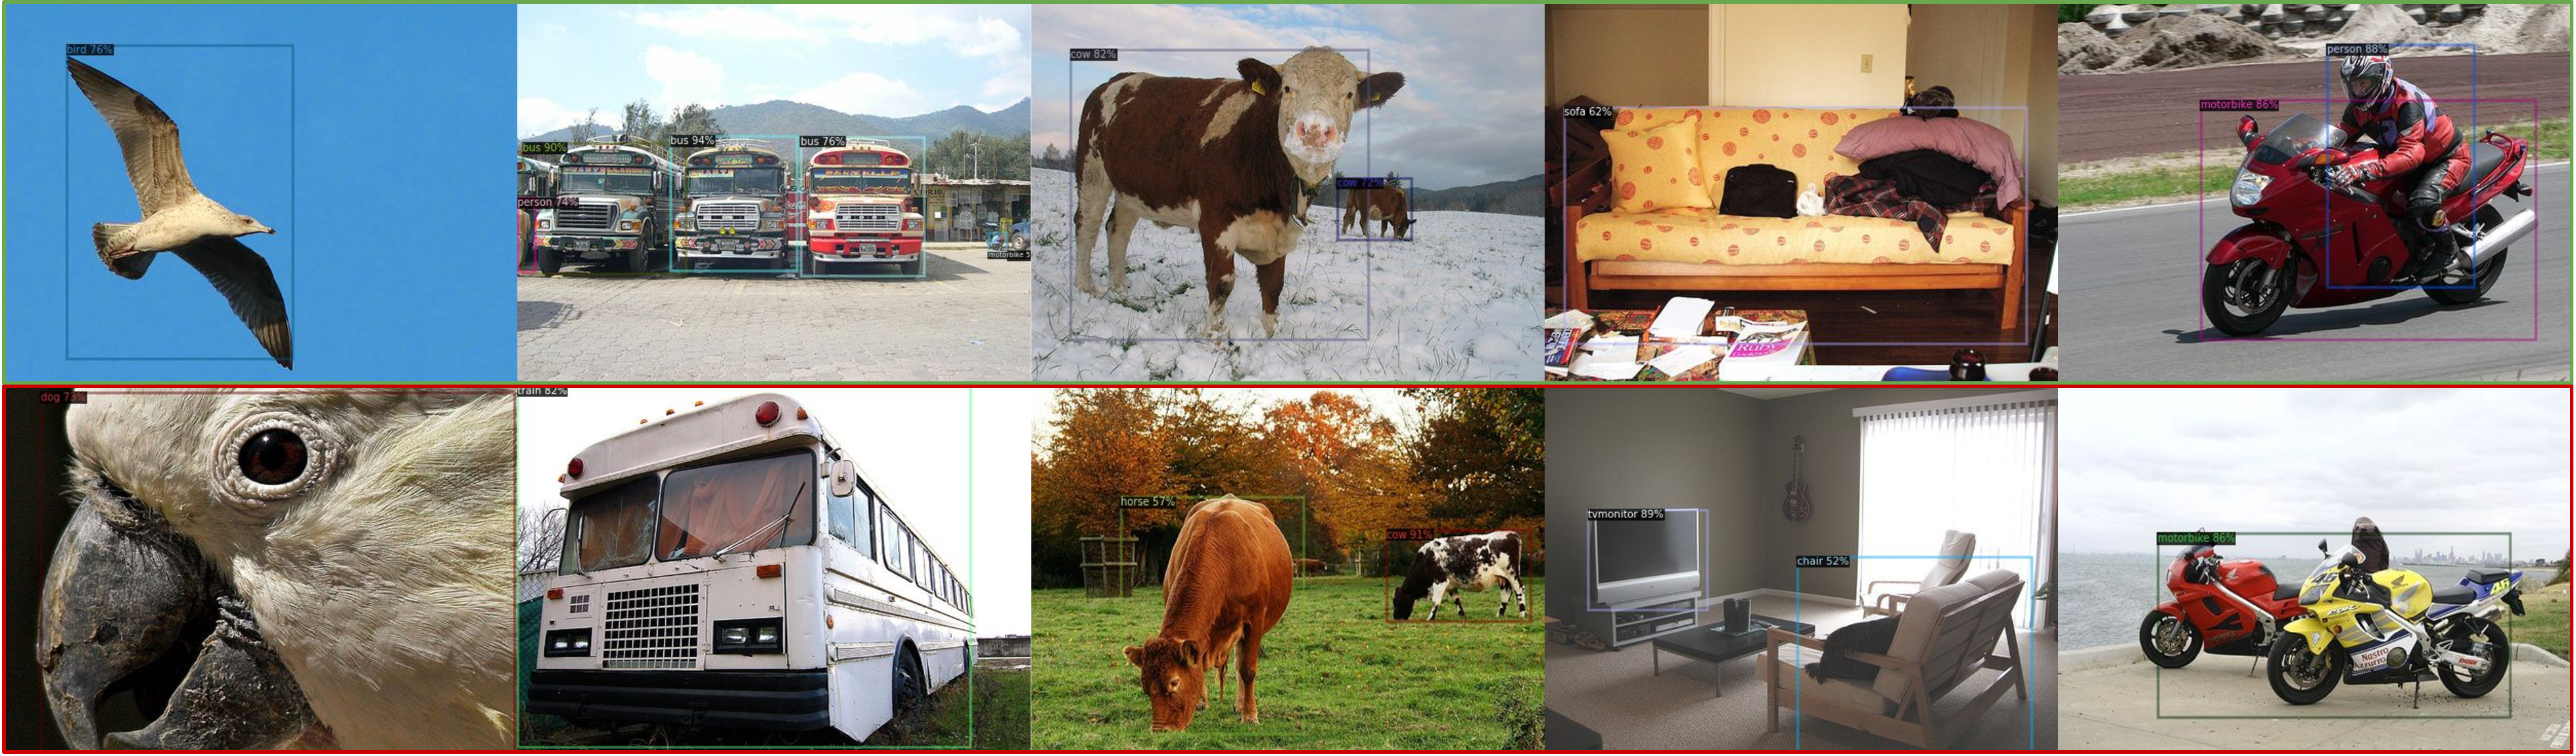
\includegraphics[width=.8\columnwidth*2]{figs/tfa_results.pdf}}
%     \caption{Detection results of our approach on novel classes (bird, bus, cow, sofa, and motorbike) from PASCAL VOC. We show success cases in the top row (green outline) and failure cases in the bottom row (red outline).}
%     \label{fig:det-vis}
%     \end{center}
%     \vspace{-8mm}
% \end{figure*}

\begin{figure*}[ht]
	\begin{center}
		\centerline{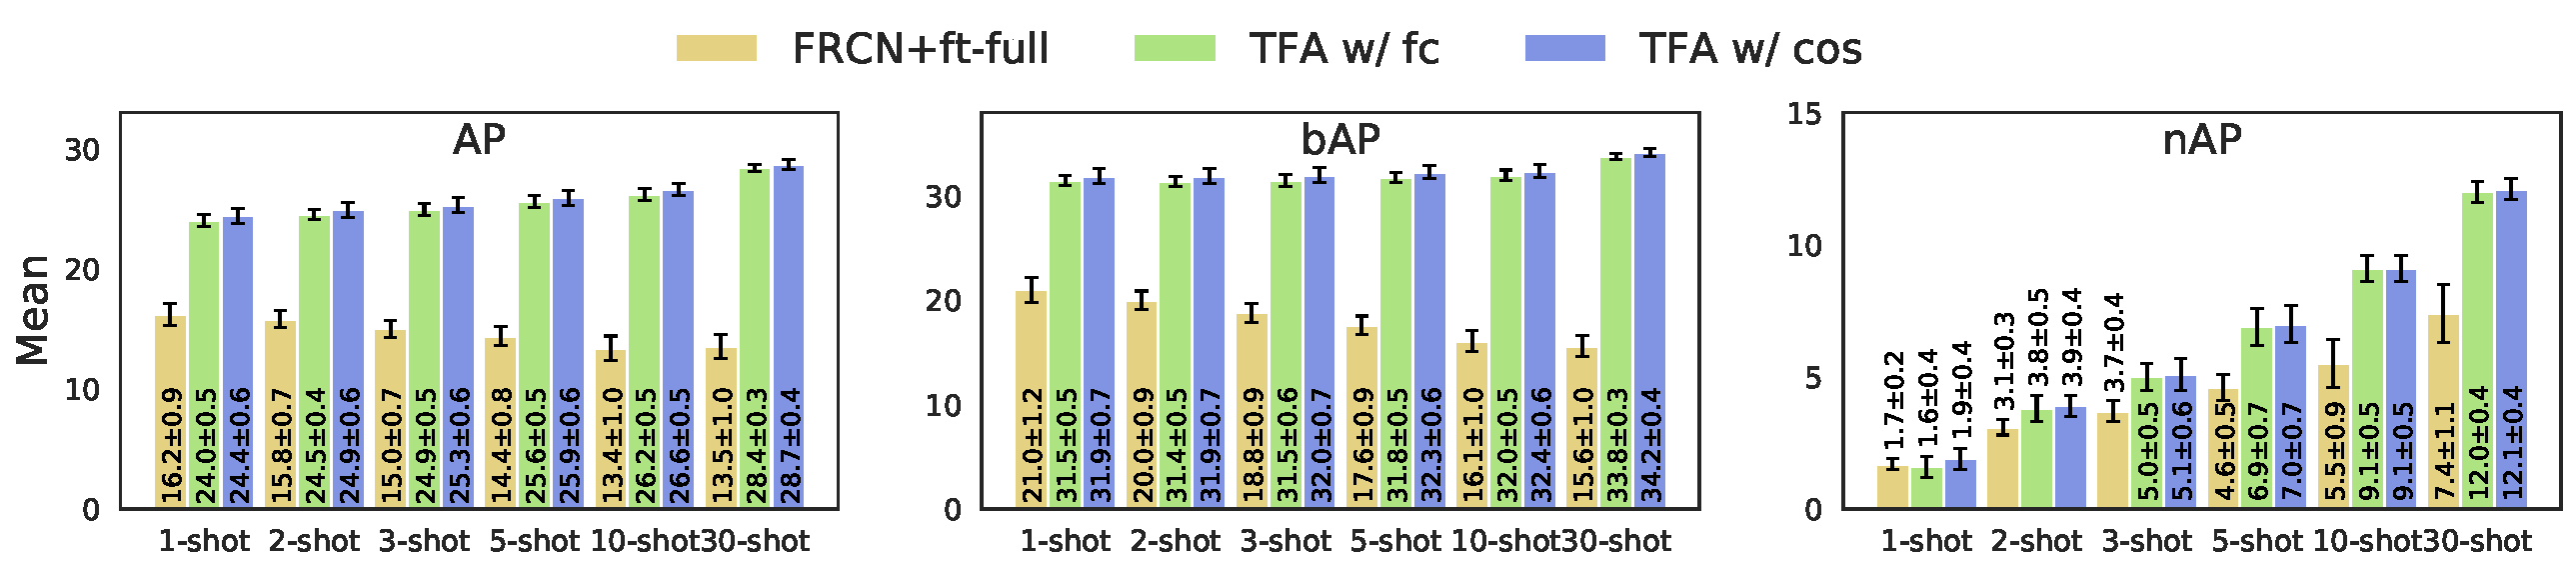
\includegraphics[width=.9\linewidth]{figs/coco_benchmark_full.pdf}}
		\vspace{-5mm}
		\caption{Generalized object detection benchmarks on COCO. For each metric, we report the average and 95\% confidence interval computed over 10 random samples.}
		\label{fig:coco_bench}
	\end{center}
\end{figure*}

{% \renewcommand{\arraystretch}{0}
\begin{figure*}[!ht]
	\centering
	\footnotesize
	\setlength{\tabcolsep}{0.1em}
	\adjustbox{width=.95\linewidth}{
		\begin{tabular}{ccccccc}
			\multirow{3}{*}{\rotatebox{90}{COCO}} &
			\rotatebox{90}{\hspace{4mm}Success} &
			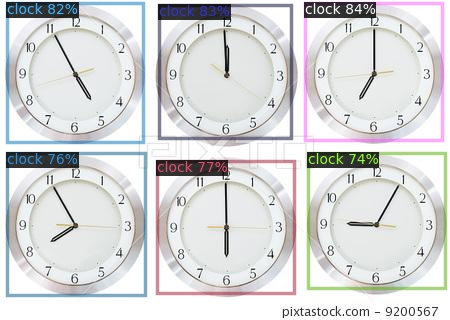
\includegraphics[width=1in]{figs/correct/clock_res.jpg} & 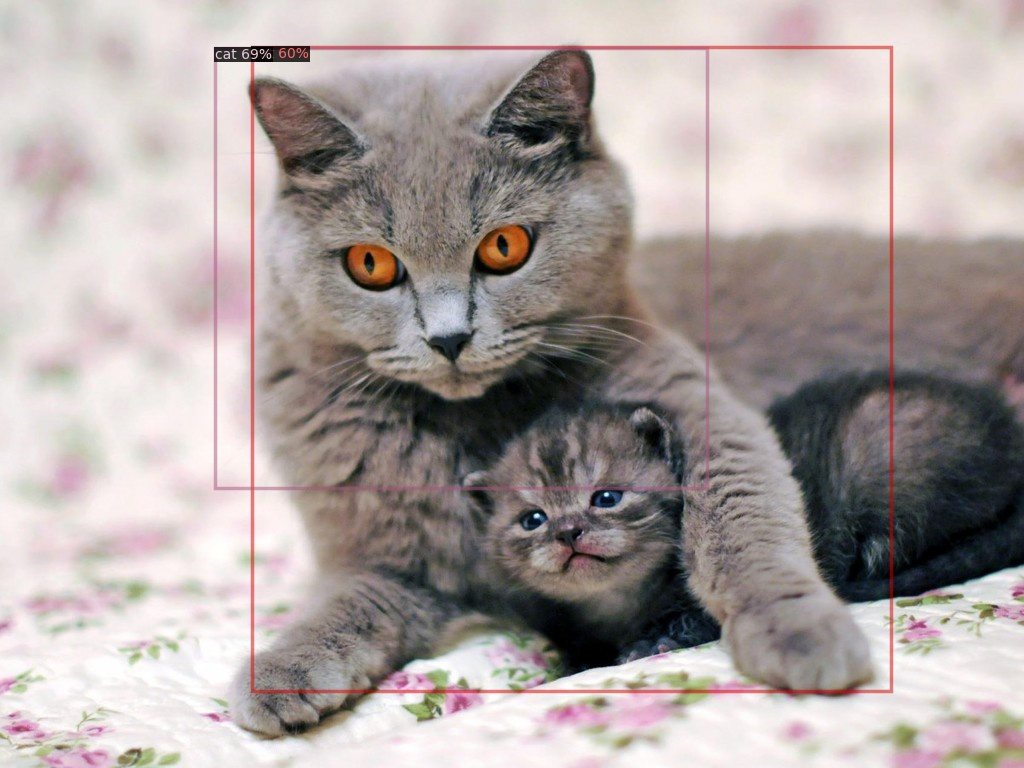
\includegraphics[width=1in]{figs/correct/miao_res.jpg} & 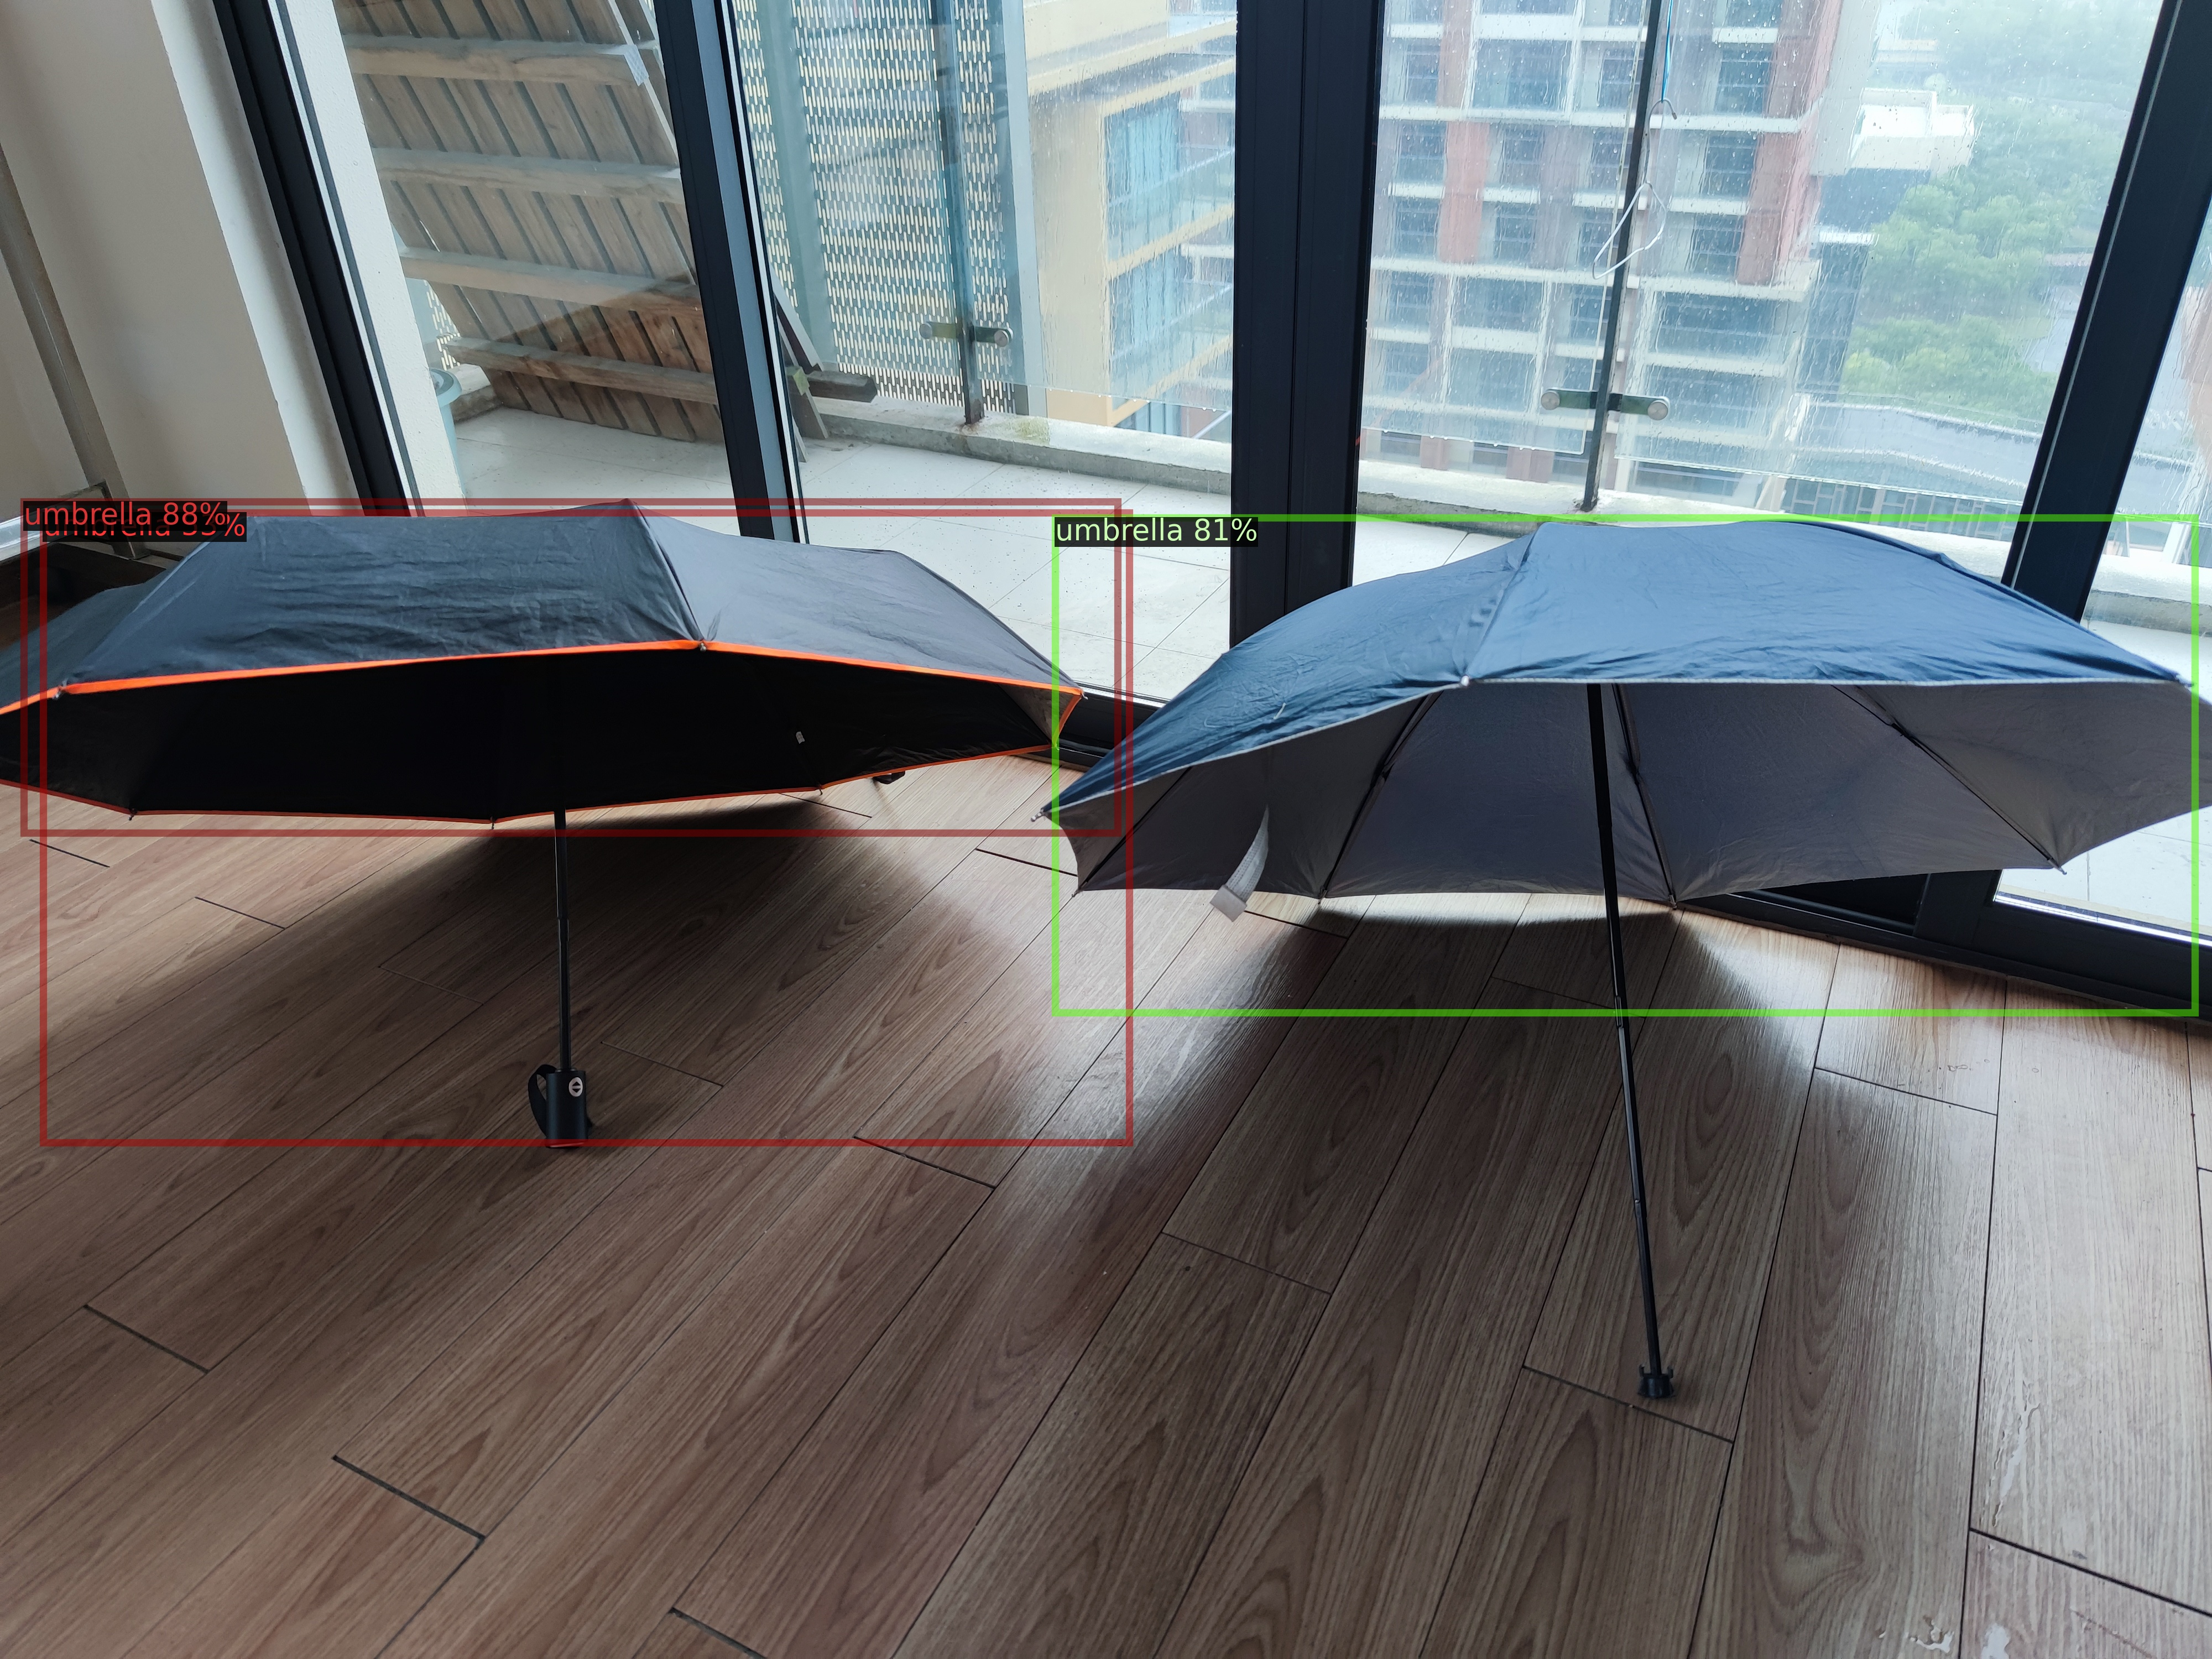
\includegraphics[width=1in]{figs/correct/2umb_res.jpg}\\
			& \rotatebox{90}{\hspace{4mm}Partial} &
			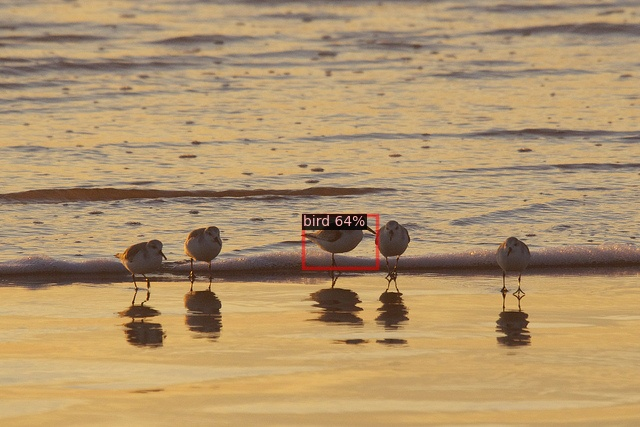
\includegraphics[width=1in]{figs/partial/bird_res.jpg} & 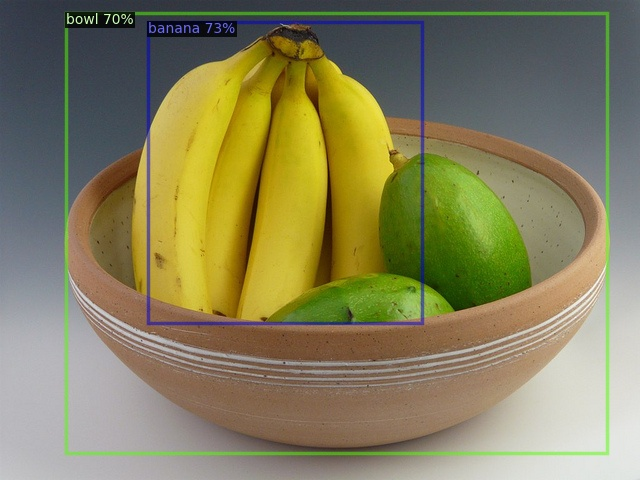
\includegraphics[width=1in]{figs/partial/fruit_res.jpg} & 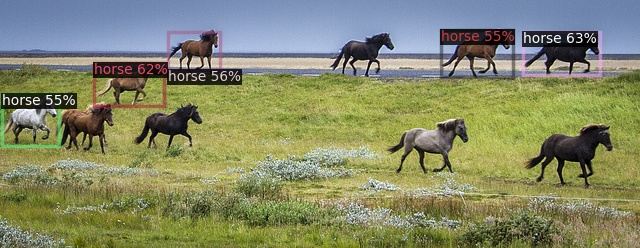
\includegraphics[width=1in]{figs/partial/horse_res.jpg}\\
			& \rotatebox{90}{\hspace{4mm}Failure} &
			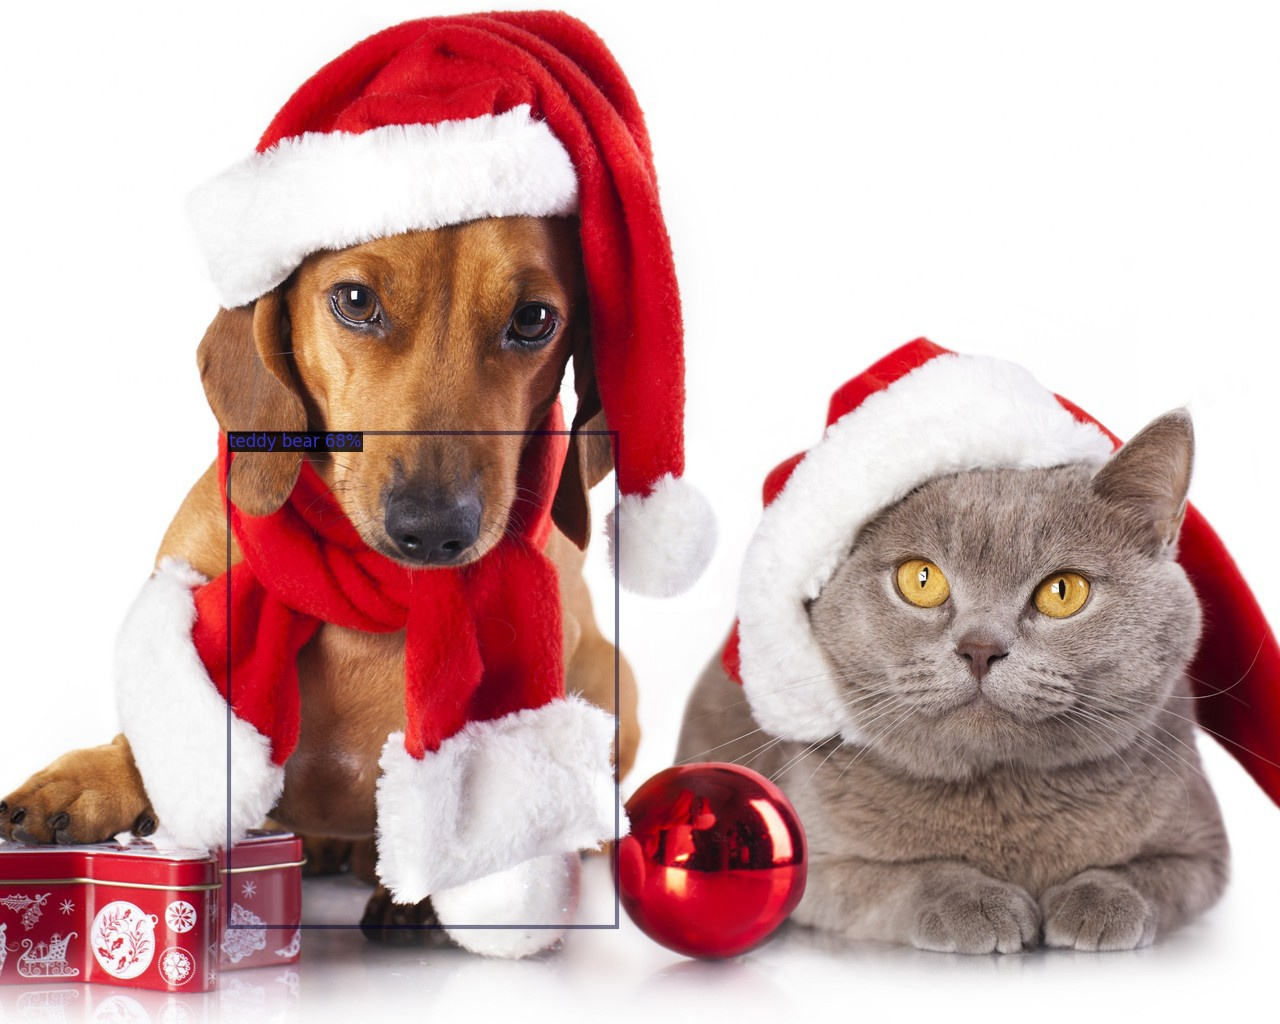
\includegraphics[width=1in]{figs/wrong/cat_dog_res.jpg} & 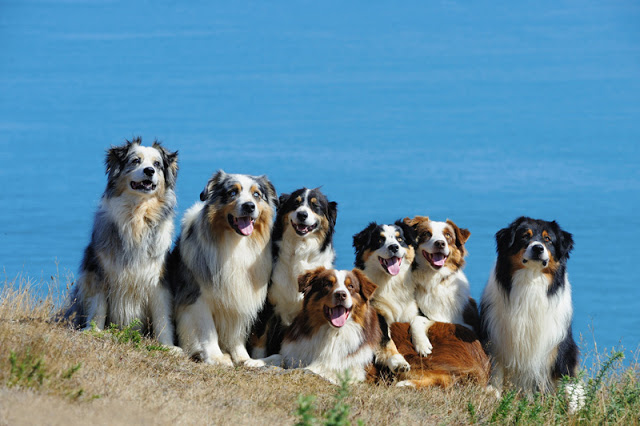
\includegraphics[width=1in]{figs/wrong/many_dogs_res.jpg} & 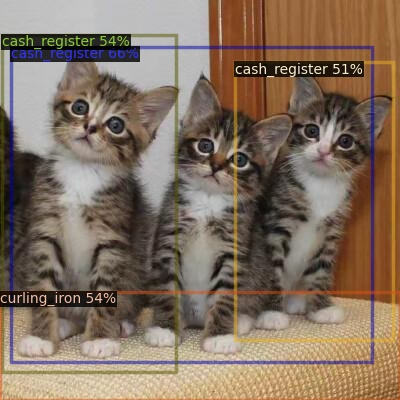
\includegraphics[width=1in]{figs/wrong/three_cat_res.jpg}\\
	\end{tabular}}
% 	\caption{Detection results of our approach on novel classes (bird, bus, cow, sofa, and motorbike) from PASCAL VOC. We show success cases (green boxes) in the top row and failure cases (red boxes) in the bottom row. \vspace{1mm}}
    \caption{Success partial and failure cases of our approach on novel classes from COCO. The black boxes are detected objects of irrelevant classes, which can be ignored. \vspace{1mm}}
    \label{fig:det-vis}
\end{figure*}}

% \minisection{More random samples.}
% On the current few-shot object detection benchmarks, performance numbers are reported and compared on a single random sample of training shots.
% However, since only a few examples are available, these numbers have high variance, and the differences in performance may vary greatly from sample to sample, thus making the comparisons unreliable.
% To address this issue, we train our models on multiple random samples of training shots to obtain means and confidence intervals, which are used for better comparisons.
% In Figure~\ref{fig:avg-ap}, we show the cumulative mean and 95\% confidence interval across 40 repeated runs on four different shots on the first split of PASCAL VOC.
% Although the performance is high on the first random sample, the average decreases significantly as more samples are used.
% Additionally, the confidence intervals across the first few runs are large, especially in the low-shot scenario.
% When we use more repeated runs, the averages stabilizes and the confidence intervals become small, which allows for better comparisons.
% On PASCAL VOC, we use 30 repeated runs. \xin{maybe combine with the comments above and shorten or split this paragraph. }

% \minisection{Inclusion of base categories.}
% We additionally evaluate our models on base categories and report AP measures on base categories as well as the mean across both novel and base categories.
% Data distributions in the real world are naturally long-tailed, and the goal of few-shot vision systems should be to achieve high accuracy on novel categories while maintaining performance on base categories.

\subsection{Ablation study and visualization}
\label{sec:vis}

\minisection{Weight initialization.}
We explore two different ways of initializing the weights of the novel classifier before few-shot fine-tuning: (1) random initialization and (2) fine-tuning a predictor on the novel set and using the classifier's weights as initialization. We compare both methods on $K=1,3,10$ on COCO and show the results in Table~\ref{tab:weight_init}. 
On COCO, using the novel weights can improve the performance over random initialization. This is probably due to the increased complexity and number of classes of COCO. We use novel initialization for all COCO and LVIS experiments.

\minisection{Scaling factor of cosine similarity.}
We explore the effect of different scaling factors for computing cosine similarity. We compare three different factors, $\alpha=10,20,50$. We use the same evaluation setting as the previous ablation study and report the results in Table~\ref{tab:cos_scale}. On COCO, $\alpha=20$ achieves better novel AP at the cost of worse base AP. Since it has the best performance on novel classes across both datasets, we use $\alpha=20$ in all of our experiments with cosine similarity.


\begin{table}[!h]
	\centering
	\footnotesize
	\setlength{\tabcolsep}{0.4em}
	%\caption{Ablation of weight initialization of the novel classifier before few-shot fine-tuning. We compare random initialization (Random) and initialization using fine-tuned novel weights (Novel). \vspace{1mm}}
	% We evaluate using base and novel AP on 1/3/10 shots on split 3 of PASCAL VOC and COCO.
	\caption{Ablation of weight initialization of the novel classifier. \vspace{2mm}}
	\adjustbox{width=.9\linewidth}{
		\begin{tabular}{ccccc|ccc}
% 			\toprule
			\multirow{2}{*}{Dataset}&\multirow{2}{*}{Init.}&\multicolumn{3}{c|}{Base AP} & \multicolumn{3}{c}{Novel AP}\\
			& & 1 & 3 & 10 & 1 & 3 & 10 \\ \midrule
			\multirow{2}{*}{COCO} & Random & 34.0 & \textbf{34.7} & \textbf{34.6} & 3.2 & 6.4 & 9.6 \\ 
			& Novel & \textbf{34.1} & \textbf{34.7} & \textbf{34.6} & \textbf{3.4} & \textbf{6.6} & \textbf{9.8} \\
			\bottomrule
	\end{tabular}}
	\label{tab:weight_init} 
\end{table}

\begin{table}[!h]
	\centering
	\footnotesize
	\setlength{\tabcolsep}{0.4em}
	\caption{Ablation of scaling factor of cosine similarity. \vspace{1mm}}
	\adjustbox{width=.9\linewidth}{
		\begin{tabular}{ccccc|ccc}
% 			\toprule
			&&\multicolumn{3}{c|}{Base AP} & \multicolumn{3}{c}{Novel AP}\\
			Dataset & Scale  & 1 & 3 & 10 & 1 & 3 & 10 \\ \midrule
			\multirow{3}{*}{COCO} & 10 & \textbf{34.3} & \textbf{34.9} & \textbf{35.0} & 2.8 & 3.4 & 4.7 \\ 
			& 20 & 34.1 & 34.7 & 33.9 & \textbf{3.4} & \textbf{6.6} & \textbf{10.0} \\
			& 50 & 30.1 & 30.7 & 34.3 & 2.4 & 5.4 & 9.0 \\
			\bottomrule
	\end{tabular}} 
	\label{tab:cos_scale}
\end{table}

\minisection{Detection results.}
We provide qualitative visualizations of the detected novel objects on COCO in Figure~\ref{fig:det-vis}.
We show both success (green boxes) and failure cases (red boxes) when detecting novel objects for COCO to help analyze the possible error types.
On COCO, we visualize the results of the 30-shot \texttt{\model w/cos} model.
The failure cases include misclassifying novel objects as similar base objects, \textit{e.g.}, row 2 columns 1, 2, 3, and 4, mislocalizing the objects, \textit{e.g.}, row 2 column 5, and missing detections, \textit{e.g.}, row 4 columns 1 and 5.
% We visualize the success and failure cases of our 10-shot \model w/ cos model on novel objects from the first split of PASCAL VOC in Figure~\ref{fig:det-vis}.
% Some failure cases include misclassifying novel objects as similar base objects, \textit{e.g.}, cow as horse, and identifying incorrect instance boundaries.

% In this section, we provide more qualitative visualization of the detected novel objects on Pascal VOC and COCO shown in Figure~\ref{fig:det-vis-sup}. We show both success (denoted by green boxes) and failure cases (denoted by red boxes) for each dataset to help analyze possible error types when detecting novel objects. The black boxes are detected objects of irrelevant classes, which can be ignored.  
% On PASCAL VOC, we visualize the results of the 10-shot \texttt{\model w/cos} model on novel objects from splits 2 and 3.
% On COCO, we visualize the results of the 30-shot \texttt{\model w/cos} model on novel objects.

% The failure cases shown in Figure~\ref{fig:det-vis-sup} could be misclassifying the object types(\textit{e.g.}, row 2 columns 1, 3, and 4), mislocalizing the objects (\textit{e.g.}, row 2 columns 2 and 5), and missing boxes (\textit{e.g.}, row 4 column 1 and row 6 columns 1 and 5).

\section{Conclusion}
In this project, we use a two-stage fine-tuning method to conquer the object detection problem, which significantly outperforms prior methods and is shown to be statisticly stable with low variance. In addition, we compared the performance after fine-tuning with the performance before fine-tuning on base classes, and it turns out that the performance on base classes are hardly hurt. Therefore, our method become the state of the art object detection method so far.



\subsubsection*{Acknowledgments}
This work was supported by Berkeley AI Research, RISE Lab, Berkeley DeepDrive and DARPA. 

% In addition to NSF CISE Expeditions Award CCF-1730628, this research is supported by gifts from Alibaba,
% Amazon Web Services, Ant Financial, Arm, CapitalOne,
% Ericsson, Facebook, Google, Huawei, Intel, Microsoft,
% Nvidia, Scotiabank, Splunk and VMware.
	
\bibliographystyle{icml2020}
\bibliography{references}

\appendix
\section{Generalized Object Detection Benchmarks}
We present the full benchmark results of PASCAL VOC (Table~\ref{tab:voc_bench}) and COCO
(Table~\ref{tab:coco_bench}) on the revised benchmark used in this work. We report the average AP, AP50 and AP75 for all the classes, base classes only, and novel classes only in the tables. For each evaluation metric, we report the average value of $n$ repeated runs with different groups of randomly sampled training shots (30 for PASCAL VOC and 10 for COCO) as well as the 95\% confidence interval estimate of the mean values.  The 95\% confidence interval is calculated by 
\begin{equation}
    95\% \; CI = 1.96 \cdot \frac{s}{\sqrt{n}},
\end{equation}
where 1.96 is the $Z$-value, $s$ is the standard deviation, and $n$ is the number of repeated runs.

We compare two of our methods, one using a FC-based classifier (\texttt{\model w/fc}) and one using a cosine similarity based classifier (\texttt{\model w/cos}). We also compare against a fine-tuning baseline \texttt{FRCN+ft-full} and against FSRW~\cite{kang2019few} using their released code on PASCAL VOC shown in Table~\ref{tab:voc_bench}. 

As shown in Table~\ref{tab:voc_bench},
\texttt{\model w/cos} is able to significantly outperform \texttt{\model w/fc} in overall AP across most splits and shots.
We observe that using a cosine similarity based classifier can achieve much higher accuracy on base classes, especially in higher shots.
On split 1 and 3, \texttt{\model w/cos} is able to outperform \texttt{\model w/fc} by over 3 points on bAP on 5 and 10 shots.
Across all shots in split 1, \texttt{\model w/cos} consistently outperforms \texttt{\model w/fc} on nAP75 by over 2 points in the novel classes. 

Moreover, the AP of our models is usually over 10 points higher than that of \texttt{FRCN+ft-full} and FSRW on all settings. Note that FSRW uses YOLOv2 as the base object detector, while we are using Faster R-CNN. ~\citet{wang2019meta} shows that there are only about 2 points of difference when using a one or two-stage detector. Therefore, our improvements should still be significant despite the difference in the base detector.

We evaluate on COCO over six different number of shots $K=1,2,3,5,10,30$ shown in Table~\ref{tab:coco_bench}.
Although the differences are less significant than on PASCAL VOC, similar observations can be made about accuracy on base classes and novel classes.

\begin{table*}[!h]
\centering
\footnotesize
\setlength{\tabcolsep}{0.4em}
\caption{Generalized object detection benchmarks on PASCAL VOC. For each metric, we report the average and 95\% confidence interval computed over 30 random samples. \vspace{1mm}}
\adjustbox{width=\linewidth}{
\begin{tabular}{c|c|c|ccc|ccc|ccc}
\toprule
\multirow{2}{*}{Split} & \multirow{2}{*}{\# shots} &\multirow{2}{*}{Method} &  \multicolumn{3}{c|}{Overall}  &\multicolumn{3}{c|}{Base class} & \multicolumn{3}{c}{Novel class} \\ \cmidrule{4-12}
& & & AP & AP50 & AP75 & bAP & bAP50 & bAP75 & nAP & nAP50 & nAP75 \\ \midrule
\multirow{21}{*}{Split 1} & 
\multirow{4}{*}{1}
    & FSRW~\cite{kang2019few} & 27.6 $ \pm $ 0.5 & 50.8 $ \pm $ 0.9 & 26.5 $ \pm $ 0.6 & 34.1 $ \pm $ 0.5 & 62.9 $ \pm $ 0.9 & 32.6 $ \pm $ 0.5 & 8.0 $ \pm $ 1.0 & 14.2 $ \pm $ 1.7 & 7.9 $ \pm $ 1.1\\
    & & FRCN+ft-full & 30.2$\pm$0.6 & 49.4$\pm$0.7 & 32.2$\pm$0.9 & 38.2$\pm$0.8 & 62.6$\pm$1.0 & 40.8$\pm$1.1 & 6.0$\pm$0.7 & 9.9$\pm$1.2 & 6.3$\pm$0.8\\
     & & {\model w/fc} & 39.6$\pm$0.5 & 63.5$\pm$0.7 & 43.2$\pm$0.7 & 48.7$\pm$0.7 & 77.1$\pm$0.7 & 53.7$\pm$1.0 & 12.2$\pm$1.6 & 22.9$\pm$2.5 & 11.6$\pm$1.9 \\
    & &\cellcolor{Gray} {\model w/cos} & \cellcolor{Gray}40.6$\pm$0.5 & \cellcolor{Gray}64.5$\pm$0.6 & \cellcolor{Gray}44.7$\pm$0.6 & \cellcolor{Gray}49.4$\pm$0.4 & \cellcolor{Gray}77.6$\pm$0.2 & \cellcolor{Gray}54.8$\pm$0.5 & \cellcolor{Gray}14.2$\pm$1.4 &\cellcolor{Gray} 25.3$\pm$2.2 & \cellcolor{Gray}14.2$\pm$1.8 \\ \cmidrule{2-12}
    & \multirow{4}{*}{2} & FSRW~\cite{kang2019few} & 
    28.7$\pm$0.4&52.2$\pm$0.6&27.7$\pm$0.5&33.9$\pm$0.4&61.8$\pm$0.5&32.7$\pm$0.5&13.2$\pm$1.0&23.6$\pm$1.7&12.7$\pm$1.1 \\
    & & FRCN+ft-full & 30.5$\pm$0.6 & 49.4$\pm$0.8 & 32.6$\pm$0.7 & 37.3$\pm$0.7 & 60.7$\pm$1.0 & 40.1$\pm$0.9 & 9.9$\pm$0.9 & 15.6$\pm$1.4 & 10.3$\pm$1.0 \\
    & & {\model w/fc} & 40.5$\pm$0.5 & 65.5$\pm$0.7 & 43.8$\pm$0.7 & 47.8$\pm$0.7 & 75.8$\pm$0.7 & 52.2$\pm$1.0 & 18.9$\pm$1.5 & 34.5$\pm$2.4 & 18.4$\pm$1.9  \\
    & &\cellcolor{Gray} {\model w/cos} & \cellcolor{Gray}42.6$\pm$0.3 & \cellcolor{Gray} 67.1$\pm$0.4 & \cellcolor{Gray}47.0$\pm$0.4 &\cellcolor{Gray} 49.6$\pm$0.3 & \cellcolor{Gray}77.3$\pm$0.2 & \cellcolor{Gray}55.0$\pm$0.4 & \cellcolor{Gray}21.7$\pm$1.0 & \cellcolor{Gray}36.4$\pm$1.6 & \cellcolor{Gray}22.8$\pm$1.3  \\ \cmidrule{2-12}
    & \multirow{4}{*}{3} & FSRW~\cite{kang2019few} & 29.5$\pm$0.3&53.3$\pm$0.6&28.6$\pm$0.4&33.8$\pm$0.3&61.2$\pm$0.6&32.7$\pm$0.4&16.8$\pm$0.9&29.8$\pm$1.6&16.5$\pm$1.0 \\
    & & FRCN+ft-full & 31.8$\pm$0.5 & 51.4$\pm$0.8 & 34.2$\pm$0.6 & 37.9$\pm$0.5 & 61.3$\pm$0.7 & 40.7$\pm$0.6 & 13.7$\pm$1.0 & 21.6$\pm$1.6 & 14.8$\pm$1.1 \\
    & & {\model w/fc} & 41.8$\pm$0.9 & 67.1$\pm$0.9 & 45.4$\pm$1.2 & 48.2$\pm$0.9 & 76.0$\pm$0.9 & 53.1$\pm$1.2 & 22.6$\pm$1.2 & 40.4$\pm$1.7 & 22.4$\pm$1.7  \\
    & & \cellcolor{Gray}{\model w/cos} &\cellcolor{Gray} 43.7$\pm$0.3 &\cellcolor{Gray} 68.5$\pm$0.4 & \cellcolor{Gray}48.3$\pm$0.4 & \cellcolor{Gray}49.8$\pm$0.3 & \cellcolor{Gray}77.3$\pm$0.2 & \cellcolor{Gray}55.4$\pm$0.4 & \cellcolor{Gray}25.4$\pm$0.9 & \cellcolor{Gray}42.1$\pm$1.5 & \cellcolor{Gray}27.0$\pm$1.2  \\ \cmidrule{2-12}
    & \multirow{4}{*}{5} & FSRW~\cite{kang2019few} & 30.4$\pm$0.3&54.6$\pm$0.5&29.6$\pm$0.4&33.7$\pm$0.3&60.7$\pm$0.4&32.8$\pm$0.4&20.6$\pm$0.8&36.5$\pm$1.4&20.0$\pm$0.9 \\
    & & FRCN+ft-full & 32.7$\pm$0.5 & 52.5$\pm$0.8 & 35.0$\pm$0.6 & 37.6$\pm$0.4 & 60.6$\pm$0.6 & 40.3$\pm$0.5 & 17.9$\pm$1.1 & 28.0$\pm$1.7 & 19.2$\pm$1.3 \\
    & & {\model w/fc} & 41.9$\pm$0.6 & 68.0$\pm$0.7 & 45.0$\pm$0.8 & 47.2$\pm$0.6 & 75.1$\pm$0.6 & 51.5$\pm$0.8 & 25.9$\pm$1.0 & 46.7$\pm$1.4 & 25.3$\pm$1.2  \\
    & &\cellcolor{Gray} {\model w/cos} &\cellcolor{Gray} 44.8$\pm$0.3 & \cellcolor{Gray}70.1$\pm$0.4 &\cellcolor{Gray} 49.4$\pm$0.4 &\cellcolor{Gray} 50.1$\pm$0.2 &\cellcolor{Gray} 77.4$\pm$0.3 &\cellcolor{Gray} 55.6$\pm$0.3 &\cellcolor{Gray} 28.9$\pm$0.8 & \cellcolor{Gray}47.9$\pm$1.2 & \cellcolor{Gray}30.6$\pm$1.0  \\ \cmidrule{2-12}
    & \multirow{3}{*}{10} & FRCN+ft-full & 33.3$\pm$0.4 & 53.8$\pm$0.6 & 35.5$\pm$0.4 & 36.8$\pm$0.4 & 59.8$\pm$0.6 & 39.2$\pm$0.4 & 22.7$\pm$0.9 & 35.6$\pm$1.5 & 24.4$\pm$1.0 \\
    & & {\model w/fc} & 42.8$\pm$0.3 & 69.5$\pm$0.4 & 46.0$\pm$0.4 & 47.3$\pm$0.3 & 75.4$\pm$0.3 & 51.6$\pm$0.4 & 29.3$\pm$0.7 & 52.0$\pm$1.1 & 29.0$\pm$0.9  \\
    & &\cellcolor{Gray} {\model w/cos} & \cellcolor{Gray}45.8$\pm$0.2 & \cellcolor{Gray}71.3$\pm$0.3 & \cellcolor{Gray}50.4$\pm$0.3 &\cellcolor{Gray} 50.4$\pm$0.2 & \cellcolor{Gray}77.5$\pm$0.2 &\cellcolor{Gray} 55.9$\pm$0.3 & \cellcolor{Gray}32.0$\pm$0.6 & \cellcolor{Gray}52.8$\pm$1.0 & \cellcolor{Gray}33.7$\pm$0.7  \\ \midrule
\multirow{21}{*}{Split 2} & \multirow{4}{*}{1} & FSRW~\cite{kang2019few} &
    28.4$\pm$0.5&51.7$\pm$0.9&27.3$\pm$0.6&35.7$\pm$0.5&64.8$\pm$0.9&34.6$\pm$0.7&6.3$\pm$0.9&12.3$\pm$1.9&5.5$\pm$0.7 \\
    & & FRCN+ft-full & 30.3$\pm$0.5 & 49.7$\pm$0.5 & 32.3$\pm$0.7 & 38.8$\pm$0.6 & 63.2$\pm$0.7 & 41.6$\pm$0.9 & 5.0$\pm$0.6 & 9.4$\pm$1.2 & 4.5$\pm$0.7 \\
    & & {\model w/fc} & 36.2$\pm$0.8 & 59.6$\pm$0.9 & 38.7$\pm$1.0 & 45.6$\pm$0.9 & 73.8$\pm$0.9 & 49.4$\pm$1.2 & 8.1$\pm$1.2 & 16.9$\pm$2.3 & 6.6$\pm$1.1  \\
    & &\cellcolor{Gray} {\model w/cos} & \cellcolor{Gray}36.7$\pm$0.6 &\cellcolor{Gray} 59.9$\pm$0.8 &\cellcolor{Gray} 39.3$\pm$0.8 &\cellcolor{Gray} 45.9$\pm$0.7 & \cellcolor{Gray}73.8$\pm$0.8 &\cellcolor{Gray} 49.8$\pm$1.1 & \cellcolor{Gray}9.0$\pm$1.2 & \cellcolor{Gray}18.3$\pm$2.4 &\cellcolor{Gray} 7.8$\pm$1.2 \\ \cmidrule{2-12}
    & \multirow{4}{*}{2} & FSRW~\cite{kang2019few} & 
    29.4$\pm$0.3&53.1$\pm$0.6&28.5$\pm$0.4&35.8$\pm$0.4&64.2$\pm$0.6&35.1$\pm$0.5&9.9$\pm$0.7&19.6$\pm$1.3&8.8$\pm$0.6 \\
    & & FRCN+ft-full & 30.7$\pm$0.5 & 49.7$\pm$0.7 & 32.9$\pm$0.6 & 38.4$\pm$0.5 & 61.6$\pm$0.7 & 41.4$\pm$0.7 & 7.7$\pm$0.8 & 13.8$\pm$1.4 & 7.4$\pm$0.8 \\
    & &{\model w/fc} & 38.5$\pm$0.5 & 62.8$\pm$0.6 & 41.2$\pm$0.6 & 46.9$\pm$0.5 & 74.9$\pm$0.5 & 51.2$\pm$0.7 & 13.1$\pm$1.0 & 26.4$\pm$1.9 & 11.3$\pm$1.1  \\
    & & \cellcolor{Gray}{\model w/cos} & \cellcolor{Gray}39.0$\pm$0.4 & \cellcolor{Gray}63.0$\pm$0.5 & \cellcolor{Gray}42.1$\pm$0.6 & \cellcolor{Gray}47.3$\pm$0.4 & \cellcolor{Gray}74.9$\pm$0.4 &\cellcolor{Gray} 51.9$\pm$0.7 &\cellcolor{Gray} 14.1$\pm$0.9 &\cellcolor{Gray} 27.5$\pm$1.6 &\cellcolor{Gray} 12.7$\pm$1.0  \\ \cmidrule{2-12}
    & \multirow{4}{*}{3} & FSRW~\cite{kang2019few} & 29.9$\pm$0.3&53.9$\pm$0.4&29.0$\pm$0.4&35.7$\pm$0.3&63.5$\pm$0.4&35.1$\pm$0.4&12.5$\pm$0.7&25.1$\pm$1.4&10.4$\pm$0.7 \\
    & & FRCN+ft-full & 31.1$\pm$0.3 & 50.1$\pm$0.5 & 33.2$\pm$0.5 & 38.1$\pm$0.4 & 61.0$\pm$0.6 & 41.2$\pm$0.5 & 9.8$\pm$0.9 & 17.4$\pm$1.6 & 9.4$\pm$1.0 \\
    & &{\model w/fc} & 39.4$\pm$0.4 & 64.2$\pm$0.5 & 42.0$\pm$0.5 & 47.5$\pm$0.4 & 75.4$\pm$0.5 & 51.7$\pm$0.6 & 15.2$\pm$0.8 & 30.5$\pm$1.5 & 13.1$\pm$0.8  \\
    & & \cellcolor{Gray}{\model w/cos} & \cellcolor{Gray}40.1$\pm$0.3 &\cellcolor{Gray} 64.5$\pm$0.5 &\cellcolor{Gray} 43.3$\pm$0.4 &\cellcolor{Gray} 48.1$\pm$0.3 & \cellcolor{Gray}75.6$\pm$0.4 & \cellcolor{Gray}52.9$\pm$0.5 & \cellcolor{Gray}16.0$\pm$0.8 & \cellcolor{Gray}30.9$\pm$1.6 & \cellcolor{Gray}14.4$\pm$0.9  \\ \cmidrule{2-12}
    & \multirow{4}{*}{5} & FSRW~\cite{kang2019few} & 30.4$\pm$0.4&54.6$\pm$0.5&29.5$\pm$0.5&35.3$\pm$0.3&62.4$\pm$0.4&34.9$\pm$0.5&15.7$\pm$0.8&31.4$\pm$1.5&13.3$\pm$0.9 \\
    & & FRCN+ft-full & 31.5$\pm$0.3 & 50.8$\pm$0.7 & 33.6$\pm$0.4 & 37.9$\pm$0.4 & 60.4$\pm$0.6 & 40.8$\pm$0.5 & 12.4$\pm$0.9 & 21.9$\pm$1.5 & 12.1$\pm$0.9 \\
    & &{\model w/fc} & 40.0$\pm$0.4 & 65.1$\pm$0.5 & 42.6$\pm$0.5 & 47.5$\pm$0.4 & 75.3$\pm$0.5 & 51.6$\pm$0.5 & 17.5$\pm$0.7 & 34.6$\pm$1.1 & 15.5$\pm$0.9  \\
    & & \cellcolor{Gray}{\model w/cos} & \cellcolor{Gray}40.9$\pm$0.4 & \cellcolor{Gray}65.7$\pm$0.5 & \cellcolor{Gray}44.1$\pm$0.5 & \cellcolor{Gray}48.6$\pm$0.4 &\cellcolor{Gray} 76.2$\pm$0.4 & \cellcolor{Gray}53.3$\pm$0.5 & \cellcolor{Gray}17.8$\pm$0.8 &\cellcolor{Gray} 34.1$\pm$1.4 & \cellcolor{Gray}16.2$\pm$1.0  \\ \cmidrule{2-12}
    & \multirow{3}{*}{10} & FRCN+ft-full & 32.2$\pm$0.3 & 52.3$\pm$0.4 & 34.1$\pm$0.4 & 37.2$\pm$0.3 & 59.8$\pm$0.4 & 39.9$\pm$0.4 & 17.0$\pm$0.8 & 29.8$\pm$1.4 & 16.7$\pm$0.9 \\
    & & {\model w/fc} & 41.3$\pm$0.2 & 67.0$\pm$0.3 & 44.0$\pm$0.3 & 48.3$\pm$0.2 & 76.1$\pm$0.3 & 52.7$\pm$0.4 & 20.2$\pm$0.5 & 39.7$\pm$0.9 & 18.0$\pm$0.7  \\
    & & \cellcolor{Gray}{\model w/cos} & \cellcolor{Gray}42.3$\pm$0.3 &\cellcolor{Gray} 67.6$\pm$0.4 &\cellcolor{Gray} 45.7$\pm$0.3 &\cellcolor{Gray} 49.4$\pm$0.2 & \cellcolor{Gray}76.9$\pm$0.3 & \cellcolor{Gray}54.5$\pm$0.3 &\cellcolor{Gray} 20.8$\pm$0.6 &\cellcolor{Gray} 39.5$\pm$1.1 & \cellcolor{Gray}19.2$\pm$0.6  \\ \midrule
\multirow{21}{*}{Split 3} & \multirow{4}{*}{1} & FSRW~\cite{kang2019few} &
27.5$\pm$0.6&50.0$\pm$1.0&26.8$\pm$0.7&34.5$\pm$0.7&62.5$\pm$1.2&33.5$\pm$0.7&6.7$\pm$1.0&12.5$\pm$1.6&6.4$\pm$1.0 \\
    & & FRCN+ft-full & 30.8$\pm$0.6 & 49.8$\pm$0.8 & 32.9$\pm$0.8 & 39.6$\pm$0.8 & 63.7$\pm$1.0 & 42.5$\pm$0.9 & 4.5$\pm$0.7 & 8.1$\pm$1.3 & 4.2$\pm$0.7 \\
    & & {\model w/fc} & 39.0$\pm$0.6 & 62.3$\pm$0.7 & 42.1$\pm$0.8 & 49.5$\pm$0.8 & 77.8$\pm$0.8 & 54.0$\pm$1.0 & 7.8$\pm$1.1 & 15.7$\pm$2.1 & 6.5$\pm$1.0 \\
    & & \cellcolor{Gray}{\model w/cos} & \cellcolor{Gray}40.1$\pm$0.3 &\cellcolor{Gray} 63.5$\pm$0.6 &\cellcolor{Gray} 43.6$\pm$0.5 &\cellcolor{Gray} 50.2$\pm$0.4 & \cellcolor{Gray}78.7$\pm$0.2 & \cellcolor{Gray}55.1$\pm$0.5 & \cellcolor{Gray}9.6$\pm$1.1 & \cellcolor{Gray}17.9$\pm$2.0 &\cellcolor{Gray} 9.1$\pm$1.2  \\ \cmidrule{2-12}
    & \multirow{4}{*}{2} & FSRW~\cite{kang2019few} & 28.7$\pm$0.4&51.8$\pm$0.7&28.1$\pm$0.5&34.5$\pm$0.4&62.0$\pm$0.7&34.0$\pm$0.5&11.3$\pm$0.7&21.3$\pm$1.0&10.6$\pm$0.8 \\
    & & FRCN+ft-full & 31.3$\pm$0.5 & 50.2$\pm$0.9 & 33.5$\pm$0.6 & 39.1$\pm$0.5 & 62.4$\pm$0.9 & 42.0$\pm$0.7 & 8.0$\pm$0.8 & 13.9$\pm$1.4 & 7.9$\pm$0.9 \\
    & &{\model w/fc} & 41.1$\pm$0.6 & 65.1$\pm$0.7 & 44.3$\pm$0.7 & 50.1$\pm$0.7 & 77.7$\pm$0.7 & 54.8$\pm$0.9 & 14.2$\pm$1.2 & 27.2$\pm$2.0 & 12.6$\pm$1.3  \\
    & & \cellcolor{Gray}{\model w/cos} & \cellcolor{Gray}41.8$\pm$0.4 &\cellcolor{Gray} 65.6$\pm$0.6 &\cellcolor{Gray} 45.3$\pm$0.4 & \cellcolor{Gray}50.7$\pm$0.3 & \cellcolor{Gray}78.4$\pm$0.2 & \cellcolor{Gray}55.6$\pm$0.4 & \cellcolor{Gray}15.1$\pm$1.3 &\cellcolor{Gray} 27.2$\pm$2.1 & \cellcolor{Gray}14.4$\pm$1.5  \\ \cmidrule{2-12}
    & \multirow{4}{*}{3} & FSRW~\cite{kang2019few} & 
    29.2$\pm$0.4&52.7$\pm$0.6&28.5$\pm$0.4&34.2$\pm$0.3&61.3$\pm$0.6&33.6$\pm$0.4&14.2$\pm$0.7&26.8$\pm$1.4&13.1$\pm$0.7 \\
    & & FRCN+ft-full & 32.1$\pm$0.5 & 51.3$\pm$0.8 & 34.3$\pm$0.6 & 39.1$\pm$0.5 & 62.1$\pm$0.7 & 42.1$\pm$0.6 & 11.1$\pm$0.9 & 19.0$\pm$1.5 & 11.2$\pm$1.0 \\
    & &{\model w/fc} & 40.4$\pm$0.5 & 65.4$\pm$0.7 & 43.1$\pm$0.7 & 47.8$\pm$0.5 & 75.6$\pm$0.5 & 52.1$\pm$0.7 & 18.1$\pm$1.0 & 34.7$\pm$1.6 & 16.2$\pm$1.3  \\
    & &\cellcolor{Gray} {\model w/cos} &\cellcolor{Gray} 43.1$\pm$0.4 & \cellcolor{Gray}67.5$\pm$0.5 & \cellcolor{Gray}46.7$\pm$0.5 & \cellcolor{Gray}51.1$\pm$0.3 &\cellcolor{Gray} 78.6$\pm$0.2 &\cellcolor{Gray} 56.3$\pm$0.4 & \cellcolor{Gray}18.9$\pm$1.1 &\cellcolor{Gray} 34.3$\pm$1.7 &\cellcolor{Gray} 18.1$\pm$1.4  \\ \cmidrule{2-12}
    & \multirow{4}{*}{5} & FSRW~\cite{kang2019few} & 
    30.1$\pm$0.3&53.8$\pm$0.5&29.3$\pm$0.4&34.1$\pm$0.3&60.5$\pm$0.4&33.6$\pm$0.4&18.0$\pm$0.7&33.8$\pm$1.4&16.5$\pm$0.8 \\
    & & FRCN+ft-full & 32.4$\pm$0.5 & 51.7$\pm$0.8 & 34.4$\pm$0.6 & 38.5$\pm$0.5 & 61.0$\pm$0.7 & 41.3$\pm$0.6 & 14.0$\pm$0.9 & 23.9$\pm$1.7 & 13.7$\pm$0.9 \\
    & & {\model w/fc} & 41.3$\pm$0.5 & 67.1$\pm$0.6 & 44.0$\pm$0.6 & 48.0$\pm$0.5 & 75.8$\pm$0.5 & 52.2$\pm$0.6 & 21.4$\pm$0.9 & 40.8$\pm$1.3 & 19.4$\pm$1.0  \\
    & & \cellcolor{Gray}{\model w/cos} & \cellcolor{Gray}44.1$\pm$0.3 &\cellcolor{Gray} 69.1$\pm$0.4 & \cellcolor{Gray}47.8$\pm$0.4 & \cellcolor{Gray}51.3$\pm$0.2 & \cellcolor{Gray}78.5$\pm$0.3 & \cellcolor{Gray}56.4$\pm$0.3 & \cellcolor{Gray}22.8$\pm$0.9 & \cellcolor{Gray}40.8$\pm$1.4 & \cellcolor{Gray}22.1$\pm$1.1  \\ \cmidrule{2-12}
    & \multirow{3}{*}{10} & FRCN+ft-full & 33.1$\pm$0.5 & 53.1$\pm$0.7 & 35.2$\pm$0.5 & 38.0$\pm$0.5 & 60.5$\pm$0.7 & 40.7$\pm$0.6 & 18.4$\pm$0.8 & 31.0$\pm$1.2 & 18.7$\pm$1.0 \\
    & & {\model w/fc} & 42.2$\pm$0.4 & 68.3$\pm$0.5 & 44.9$\pm$0.6 & 48.5$\pm$0.4 & 76.2$\pm$0.4 & 52.9$\pm$0.5 & 23.3$\pm$0.8 & 44.6$\pm$1.1 & 21.0$\pm$1.2  \\
    & & \cellcolor{Gray}{\model w/cos} & \cellcolor{Gray}45.0$\pm$0.3 & \cellcolor{Gray}70.3$\pm$0.4 &\cellcolor{Gray} 48.9$\pm$0.4 &\cellcolor{Gray} 51.6$\pm$0.2 &\cellcolor{Gray} 78.6$\pm$0.2 &\cellcolor{Gray} 57.0$\pm$0.3 & \cellcolor{Gray}25.4$\pm$0.7 & \cellcolor{Gray}45.6$\pm$1.1 & \cellcolor{Gray}24.7$\pm$1.1  \\
\bottomrule
\end{tabular}}
\label{tab:voc_bench}
\end{table*}

\begin{table*}[ht]
\centering
\footnotesize
\setlength{\tabcolsep}{0.4em}
\caption{Generalized object detection benchmarks on COCO. For each metric, we report the average and 95\% confidence interval computed over 10 random samples. \vspace{1mm}}
\adjustbox{width=\linewidth}{
\begin{tabular}{c|c|cccccc|ccc|ccc}
\toprule
\multirow{2}{*}{\# shots} &\multirow{2}{*}{Method} &  \multicolumn{6}{c|}{Overall}  &\multicolumn{3}{c|}{Base class} & \multicolumn{3}{c}{Novel class} \\ \cmidrule{3-14}
&  & AP & AP50 & AP75 & APs & APm & APl & bAP & bAP50 & bAP75 & nAP & nAP50 & nAP75 \\ \midrule
\multirow{3}{*}{1} & FRCN+ft-full & 16.2$\pm$0.9 & 25.8$\pm$1.2 & 17.6$\pm$1.0 & 7.2$\pm$0.6 & 17.9$\pm$1.0 & 23.1$\pm$1.1 & 21.0$\pm$1.2 & 33.3$\pm$1.7 & 23.0$\pm$1.4 & 1.7$\pm$0.2 & 3.3$\pm$0.3 & 1.6$\pm$0.2 \\
 & {\model w/fc} & 24.0$\pm$0.5 & 38.9$\pm$0.5 & 25.8$\pm$0.6 & 13.8$\pm$0.4 & 26.6$\pm$0.4 & 32.0$\pm$0.6 & 31.5$\pm$0.5 & 50.7$\pm$0.6 & 33.9$\pm$0.8 & 1.6$\pm$0.4 & 3.4$\pm$0.6 & 1.3$\pm$0.4 \\
 & {\cellcolor{Gray} \model w/cos} &  \cellcolor{Gray}24.4$\pm$0.6 & \cellcolor{Gray}39.8$\pm$0.8 & \cellcolor{Gray}26.1$\pm$0.8 & \cellcolor{Gray}14.7$\pm$0.7 & \cellcolor{Gray}26.8$\pm$0.5 & \cellcolor{Gray}31.4$\pm$0.7 & \cellcolor{Gray}31.9$\pm$0.7 & \cellcolor{Gray}51.8$\pm$0.9 & \cellcolor{Gray}34.3$\pm$0.9 & \cellcolor{Gray}1.9$\pm$0.4 & \cellcolor{Gray}3.8$\pm$0.6 & \cellcolor{Gray}1.7$\pm$0.5 \\ \midrule
\multirow{3}{*}{2} & FRCN+ft-full & 15.8$\pm$0.7 & 25.0$\pm$1.1 & 17.3$\pm$0.7 & 6.6$\pm$0.6 & 17.2$\pm$0.8 & 23.5$\pm$0.7 & 20.0$\pm$0.9 & 31.4$\pm$1.5 & 22.2$\pm$1.0 & 3.1$\pm$0.3 & 6.1$\pm$0.6 & 2.9$\pm$0.3 \\
 & {\model w/fc} & 24.5$\pm$0.4 & 39.3$\pm$0.6 & 26.5$\pm$0.5 & 13.9$\pm$0.3 & 27.1$\pm$0.5 & 32.7$\pm$0.7 & 31.4$\pm$0.5 & 49.8$\pm$0.7 & 34.3$\pm$0.6 & 3.8$\pm$0.5 & 7.8$\pm$0.8 & 3.2$\pm$0.6 \\
 & {\cellcolor{Gray} \model w/cos} & \cellcolor{Gray}24.9$\pm$0.6 & \cellcolor{Gray}40.1$\pm$0.9 & \cellcolor{Gray}27.0$\pm$0.7 & \cellcolor{Gray}14.9$\pm$0.7 & \cellcolor{Gray}27.3$\pm$0.6 & \cellcolor{Gray}32.3$\pm$0.6 & \cellcolor{Gray}31.9$\pm$0.7 & \cellcolor{Gray}50.8$\pm$1.1 & \cellcolor{Gray}34.8$\pm$0.8 & \cellcolor{Gray}3.9$\pm$0.4 & \cellcolor{Gray}7.8$\pm$0.7 & \cellcolor{Gray}3.6$\pm$0.6 \\ \midrule
\multirow{3}{*}{3} & FRCN+ft-full & 15.0$\pm$0.7 & 23.9$\pm$1.2 & 16.4$\pm$0.7 & 6.0$\pm$0.6 & 16.1$\pm$0.9 & 22.6$\pm$0.9 & 18.8$\pm$0.9 & 29.5$\pm$1.5 & 20.7$\pm$0.9 & 3.7$\pm$0.4 & 7.1$\pm$0.8 & 3.5$\pm$0.4 \\
 & {\model w/fc} & 24.9$\pm$0.5 & 39.7$\pm$0.7 & 27.1$\pm$0.6 & 14.1$\pm$0.4 & 27.5$\pm$0.6 & 33.4$\pm$0.8 & 31.5$\pm$0.6 & 49.6$\pm$0.7 & 34.6$\pm$0.7 & 5.0$\pm$0.5 & 9.9$\pm$1.0 & 4.6$\pm$0.6 \\
 & {\cellcolor{Gray} \model w/cos} & \cellcolor{Gray}25.3$\pm$0.6 & \cellcolor{Gray}40.4$\pm$1.0 & \cellcolor{Gray}27.6$\pm$0.7 & \cellcolor{Gray}14.8$\pm$0.7 & \cellcolor{Gray}27.7$\pm$0.6 & \cellcolor{Gray}33.1$\pm$0.7 & \cellcolor{Gray}32.0$\pm$0.7 & \cellcolor{Gray}50.5$\pm$1.0 & \cellcolor{Gray}35.1$\pm$0.7 & \cellcolor{Gray}5.1$\pm$0.6 & \cellcolor{Gray}9.9$\pm$0.9 & \cellcolor{Gray}4.8$\pm$0.6 \\ \midrule
\multirow{3}{*}{5} & FRCN+ft-full & 14.4$\pm$0.8 & 23.0$\pm$1.3 & 15.6$\pm$0.8 & 5.6$\pm$0.4 & 15.2$\pm$1.0 & 21.9$\pm$1.1 & 17.6$\pm$0.9 & 27.8$\pm$1.5 & 19.3$\pm$1.0 & 4.6$\pm$0.5 & 8.7$\pm$1.0 & 4.4$\pm$0.6 \\
 & {\model w/fc} & 25.6$\pm$0.5 & 40.7$\pm$0.8 & 28.0$\pm$0.5 & 14.3$\pm$0.4 & 28.2$\pm$0.6 & 34.4$\pm$0.6 & 31.8$\pm$0.5 & 49.8$\pm$0.7 & 35.2$\pm$0.5 & 6.9$\pm$0.7 & 13.4$\pm$1.2 & 6.3$\pm$0.8 \\
 & {\cellcolor{Gray} \model w/cos} & \cellcolor{Gray}25.9$\pm$0.6 & \cellcolor{Gray}41.2$\pm$0.9 & \cellcolor{Gray}28.4$\pm$0.6 & \cellcolor{Gray}15.0$\pm$0.6 & \cellcolor{Gray}28.3$\pm$0.5 & \cellcolor{Gray}34.1$\pm$0.6 & \cellcolor{Gray}32.3$\pm$0.6 & \cellcolor{Gray}50.5$\pm$0.9 & \cellcolor{Gray}35.6$\pm$0.6 & \cellcolor{Gray}7.0$\pm$0.7 & \cellcolor{Gray}13.3$\pm$1.2 & \cellcolor{Gray}6.5$\pm$0.7 \\ \midrule
\multirow{3}{*}{10} & FRCN+ft-full & 13.4$\pm$1.0 & 21.8$\pm$1.7 & 14.5$\pm$0.9 & 5.1$\pm$0.4 & 14.3$\pm$1.2 & 20.1$\pm$1.5 & 16.1$\pm$1.0 & 25.7$\pm$1.8 & 17.5$\pm$1.0 & 5.5$\pm$0.9 & 10.0$\pm$1.6 & 5.5$\pm$0.9 \\
 & {\model w/fc} & 26.2$\pm$0.5 & 41.8$\pm$0.7 & 28.6$\pm$0.5 & 14.5$\pm$0.3 & 29.0$\pm$0.5 & 35.2$\pm$0.6 & 32.0$\pm$0.5 & 49.9$\pm$0.7 & 35.3$\pm$0.6 & 9.1$\pm$0.5 & 17.3$\pm$1.0 & 8.5$\pm$0.5 \\
 & {\cellcolor{Gray} \model w/cos} & \cellcolor{Gray}26.6$\pm$0.5 & \cellcolor{Gray}42.2$\pm$0.8 & \cellcolor{Gray}29.0$\pm$0.6 & \cellcolor{Gray}15.0$\pm$0.5 & \cellcolor{Gray}29.1$\pm$0.4 & \cellcolor{Gray}35.2$\pm$0.5 & \cellcolor{Gray}32.4$\pm$0.6 & \cellcolor{Gray}50.6$\pm$0.9 & \cellcolor{Gray}35.7$\pm$0.7 & \cellcolor{Gray}9.1$\pm$0.5 & \cellcolor{Gray}17.1$\pm$1.1 & \cellcolor{Gray}8.8$\pm$0.5 \\ \midrule
\multirow{3}{*}{30} & FRCN+ft-full & 13.5$\pm$1.0 & 21.8$\pm$1.9 & 14.5$\pm$1.0 & 5.1$\pm$0.3 & 14.6$\pm$1.2 & 19.9$\pm$2.0 & 15.6$\pm$1.0 & 24.8$\pm$1.8 & 16.9$\pm$1.0 & 7.4$\pm$1.1 & 13.1$\pm$2.1 & 7.4$\pm$1.0 \\
 & {\model w/fc} & 28.4$\pm$0.3 & 44.4$\pm$0.6 & 31.2$\pm$0.3 & 15.7$\pm$0.3 & 31.2$\pm$0.3 & 38.6$\pm$0.4 & 33.8$\pm$0.3 & 51.8$\pm$0.6 & 37.6$\pm$0.4 & 12.0$\pm$0.4 & 22.2$\pm$0.6 & 11.8$\pm$0.4 \\
 & {\cellcolor{Gray} \model w/cos} & \cellcolor{Gray}28.7$\pm$0.4 & \cellcolor{Gray}44.7$\pm$0.7 & \cellcolor{Gray}31.5$\pm$0.4 & \cellcolor{Gray}16.1$\pm$0.4 & \cellcolor{Gray}31.2$\pm$0.3 & \cellcolor{Gray}38.4$\pm$0.4 & \cellcolor{Gray}34.2$\pm$0.4 & \cellcolor{Gray}52.3$\pm$0.7 & \cellcolor{Gray}38.0$\pm$0.4 & \cellcolor{Gray}12.1$\pm$0.4 & \cellcolor{Gray}22.0$\pm$0.7 & \cellcolor{Gray}12.0$\pm$0.5 \\
\bottomrule
\end{tabular}}
\vspace{-1mm}
\label{tab:coco_bench}
\end{table*}

\section{Performance over Multiple Runs}
In our revised benchmark, we adopt $n$ repeated runs with different randomly sampled training shots to increase the reliability of the benchmark. In our experiments, we adopt $n=30$ for PASCAL VOC and $n=10$ for COCO. 

In this section, we provide plots of cumulative means with 95\% confidence intervals of the repeated runs to show
that the selected value of $n$ is sufficient to provide statistically stable results. 

We plot the model performance measured by AP, AP50 and AP75 of up to 40 random groups of training shots across all three splits in Figure~\ref{fig:avg-ap-sup}. For COCO, we plot  up  to  10  random  groups of training shots in Figure~\ref{fig:coco-avg-ap-sup}.

As we can observe from both Figure~\ref{fig:avg-ap-sup} and Figure~\ref{fig:coco-avg-ap-sup}, after around 30 runs on PASCAL VOC and 8 runs on COCO, the means and variances stabilize and our selected values of $n$ are sufficient to obtain stable estimates of the model performances and reliable comparisons across different methods. 

We also observe that the average value across multiple runs is consistently lower than that on the first run, especially in the one-shot case. For example, the average AP50 across 40 runs is around 15 points lower than the AP50 on the first run in the 1-shot case on split 1 on PASCAL VOC. This indicates that the accuracies on the first run, adopted by the previous work~\cite{kang2019few, yan2019meta, wang2019meta}, often overestimate the actual performance and thus lead to unreliable comparison between different approaches. 


\begin{figure*}[ht]
	\begin{center}
		\centerline{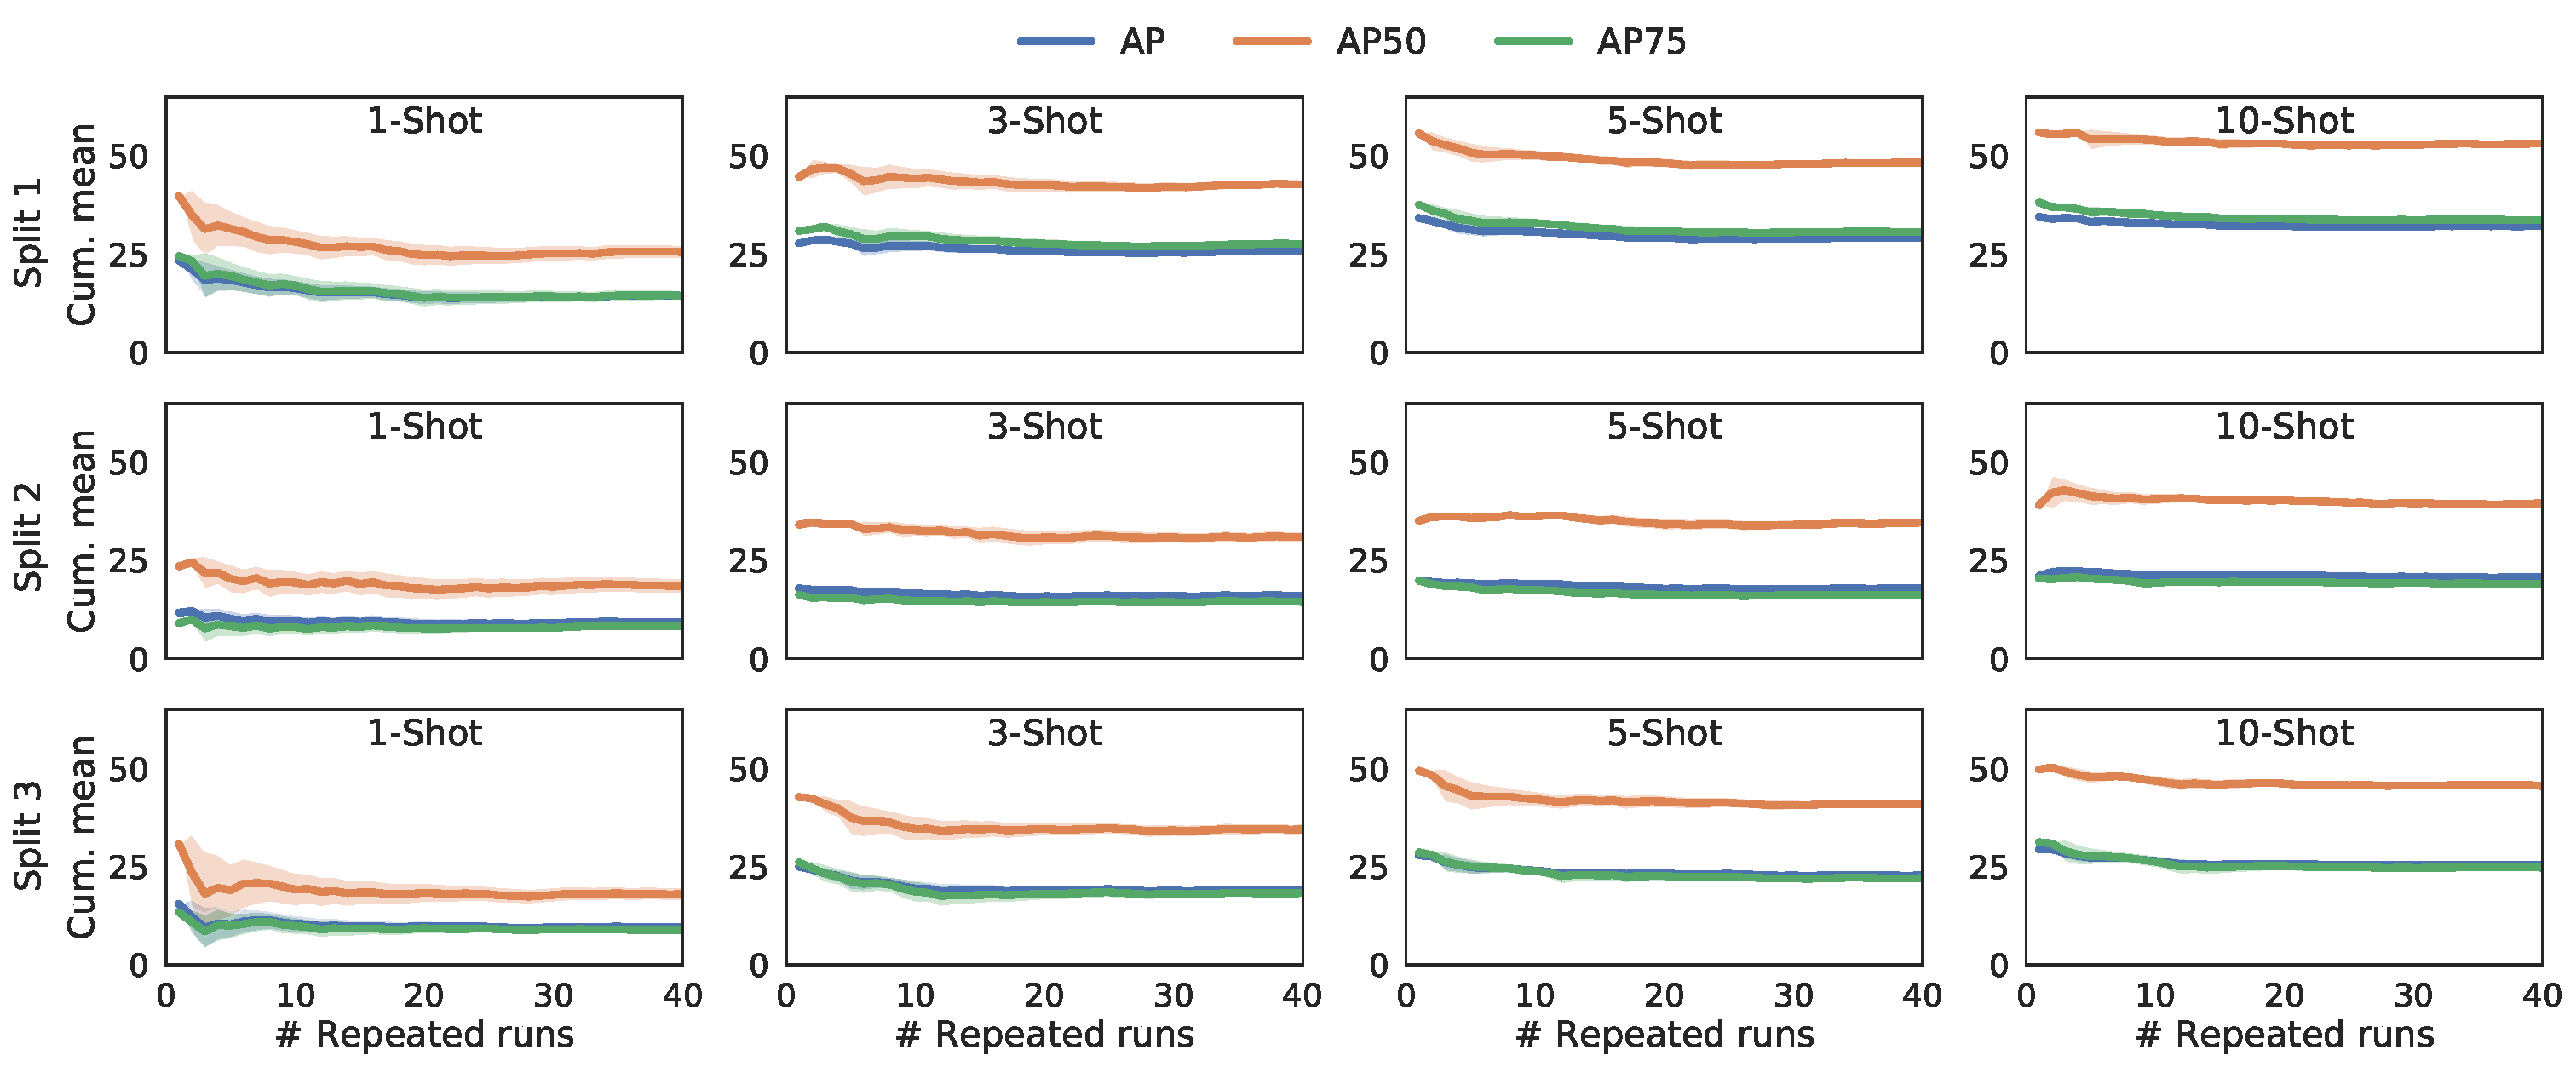
\includegraphics[width=\columnwidth*2]{figs/all_avgap_std.pdf}}
		\vspace{-5mm}
		\caption{Cumulative means with 95\% confidence intervals across 40 repeated runs, computed on the novel classes of all three splits of PASCAL VOC. The means and variances become stable after around 30 runs.}
		\label{fig:avg-ap-sup}
	\end{center}
	\vspace{-10mm}
\end{figure*}

\begin{figure*}[ht]
	\begin{center}
		\centerline{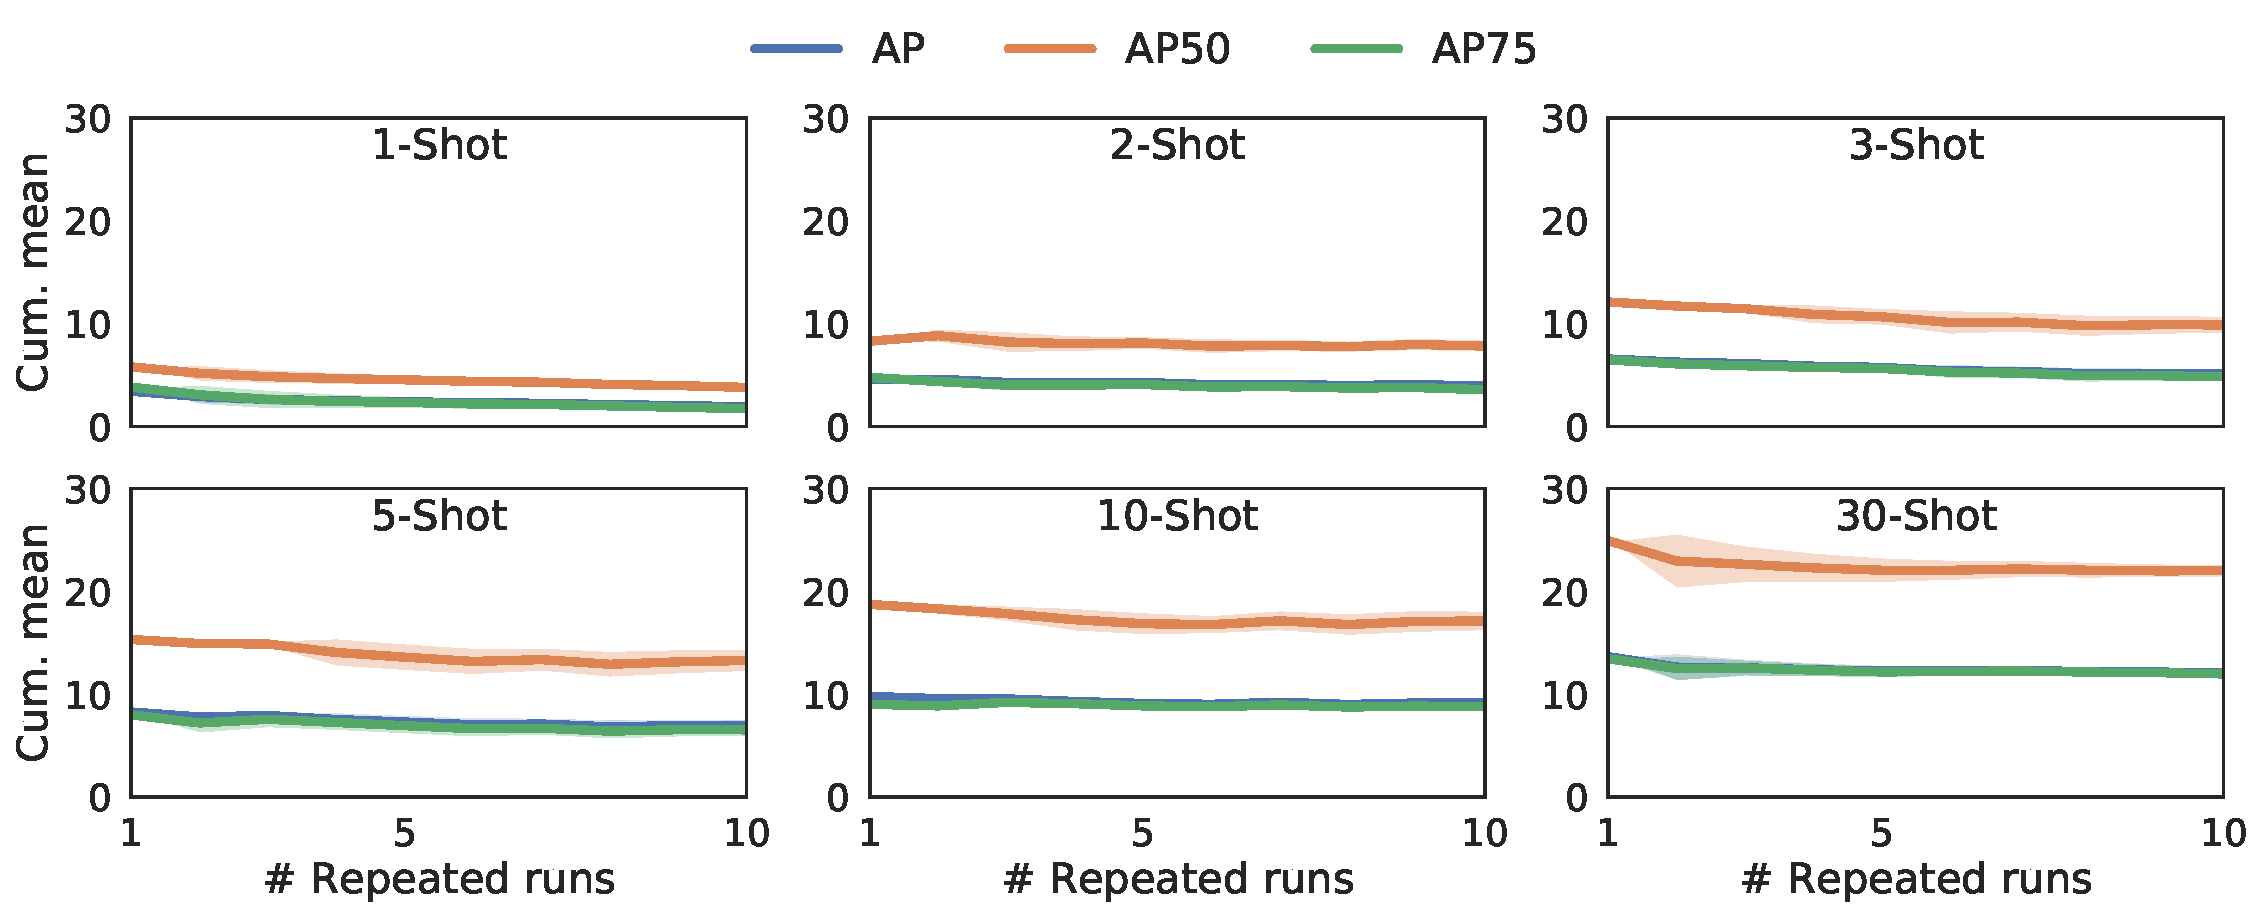
\includegraphics[width=.8\linewidth]{figs/coco_avgap_std.pdf}}
		\vspace{-5mm}
		\caption{Cumulative means with 95\% confidence intervals across 10 repeated runs, computed on the novel classes of COCO.}
		\label{fig:coco-avg-ap-sup}
	\end{center}
	\vspace{-10mm}
\end{figure*}



\end{document}


% This document was modified from the file originally made available by
% Pat Langley and Andrea Danyluk for ICML-2K. This version was created
% by Iain Murray in 2018, and modified by Alexandre Bouchard in
% 2019 and 2020. Previous contributors include Dan Roy, Lise Getoor and Tobias
% Scheffer, which was slightly modified from the 2010 version by
% Thorsten Joachims & Johannes Fuernkranz, slightly modified from the
% 2009 version by Kiri Wagstaff and Sam Roweis's 2008 version, which is
% slightly modified from Prasad Tadepalli's 2007 version which is a
% lightly changed version of the previous year's version by Andrew
% Moore, which was in turn edited from those of Kristian Kersting and
% Codrina Lauth. Alex Smola contributed to the algorithmic style files.
